% This is a general template file for the LaTeX package SVJour3
% for Springer journals. Original by Springer Heidelberg, 2010/09/16
%
% Use it as the basis for your article. Delete % signs as needed.
%
% This template includes a few options for different layouts and
% content for various journals. Please consult a previous issue of
% your journal as needed.
%
\RequirePackage{fix-cm}
%
%\documentclass{svjour3}                     % onecolumn (standard format)
%\documentclass[smallcondensed]{svjour3}     % onecolumn (ditto)
\documentclass[smallextended]{svjour3}       % onecolumn (second format)
%\documentclass[twocolumn]{svjour3}          % twocolumn
%
\smartqed  % flush right qed marks, e.g. at end of proof
%
%Line numbering (comment out when done editing)
\usepackage{lineno}
\linenumbers
%
% insert here the call for the packages your document requires
\usepackage{graphicx}
\usepackage{multirow}
\usepackage{array}
\usepackage{xcolor,tabularx}
\usepackage{rotating}
\setlength{\rotFPtop}{0pt plus 1fil}
%Bilbiography stuff
\bibliographystyle{spbasic}
\usepackage{hyperref}
\usepackage[round,authoryear]{natbib}
%Formatting stuff
\usepackage{amssymb}
\usepackage{amsmath}
\numberwithin{equation}{section}
\usepackage[title]{appendix}
\usepackage{subcaption}
\usepackage{mathptmx}      % use Times fonts if available on your TeX system
\usepackage{latexsym}
\usepackage{ulem}
% etc.
%
\newcolumntype{L}[1]{>{\raggedright\let\newline\\\arraybackslash\hspace{0pt}}p{#1}}
\newcolumntype{C}[1]{>{\centering\let\newline\\\arraybackslash\hspace{0pt}}p{#1}}
\newcolumntype{R}[1]{>{\raggedleft\let\newline\\\arraybackslash\hspace{0pt}}p{#1}}

 \journalname{Climate Dynamics}
%
\begin{document}

\title{Atmospheric Blocking and Intercomparison of Objective Detection Methods: Flow Field Characteristics
\thanks{The material is based upon work supported by NASA under award No. NNX16AG62G.  Additional support comes from the USDA National Institute of Food and Agriculture, Hatch project Accession no. 1001953 and 1010971. Authors Ullrich and Grotjahn are further supported by Department of Energy Office of Science award number DE-SC0016605, ``An Integrated Evaluation of the Simulated Hydroclimate System of the Continental US.''}
}
% Grants or other notes about the article that should go on the front
% page should be placed within the \thanks{} command in the title
% (and the %-sign in front of \thanks{} should be deleted)
%
% General acknowledgments should be placed at the end of the article.


\titlerunning{Atmospheric Blocking and Intercomparison of Objective Detection Methods}        % if too long for running head

\author{M.C.~Pinheiro\and
        P.A.~Ullrich \and 
        R.~Grotjahn
}

%\authorrunning{Short form of author list} % if too long for running head
\institute{M. C. Pinheiro \and P. A. Ullrich \and R. Grotjahn \at
              Department of Land, Air, and Water Resources, University of California, Davis, 1 Shields Ave, Davis, California, United States \\
              \email{mcpinheiro@ucdavis.edu}           %  \\
%             \emph{Present address:} of F. Author  %  if needed
           \and
           P. A. Ullrich \at
             Lawrence Berkeley National Laboratory, 1 Cyclotron Rd, Berkeley, California, United States          }



\date{Received: date / Accepted: date}
% The correct dates will be entered by the editor

\maketitle

\begin{abstract}
Objective methods for identifying and quantifying atmospheric blocking have been developed over recent decades, primarily targeting North Atlantic blocks. Differences arise from these methods, leading to changes in the resultant blocking climatology. To understand these differences, and better inform future assessments built on quantitative detection of blocks, this paper examines blocking properties produced by three different objective detection algorithms over the global extratropics.  Blocking criteria examined include 500 hPa geopotential height anomaly ($Z^*$), column-averaged potential vorticity anomaly ($PV^*$), and 500 hPa geopotential height gradient ($AGP$). Results are analyzed for blocking climatologies and for instantaneous blocking patterns, as well as distributions of block size, speed, duration, and distance traveled. The results emphasize physical characteristics of the flow field and the subsequent blocking regions that emerge; overall, $PV^*$ and $Z^*$ blocked regions often have higher pattern correlation and spatial similarity, {\color{blue}though agreement with $AGP$ can be large in some instances.}
{\color{teal}\sout{R2: unclear}}
{\color{blue}$Z^*$ finds the largest (and greatest number of) blocked regions, while $PV^*$-detected regions are smallest in the Northern and $AGP$-detected regions are smallest in the Southern Hemisphere}
{\color{teal}\sout{R2: unclear}}
. In some cases, $PV^*$ tracks a nearby jet streak, leading to differences with height-based algorithms.  All three algorithms detect some questionable low-latitude blocks that are stationary and persist but do not impair zonal flow, although at different times.  Therefore, careful consideration of the algorithm biases is important in future blocking studies. For example, linking extreme weather to detected blocking could vary substantially depending on the algorithm used.


\keywords{Blocking \and Objective detection \and Climate variability \and Climatology}
% \PACS{PACS code1 \and PACS code2 \and more}
% \subclass{MSC code1 \and MSC code2 \and more}
\end{abstract}

\section{Introduction}
\label{intro}
{\color{purple}R1: Did the authors consider some measure of block intensity as a parameter?}
Atmospheric blocking is a synoptic-scale weather phenomenon with important social and ecological impacts that arise due to its correlation with many kinds of extreme weather, such as heat waves \citep{pfahl_quantifying_2012,grotjahn_identifying_2011,lee_california_2015}, cold spells \citep{sillmann_extreme_2011,grotjahn_composite_2008}, and floods \citep{houze_anomalous_2011,hong_roles_2011}.  Yet it is a phenomenon that is not fully understood in terms of the underlying physics.  The American Meteorological Society (AMS) definition of blocking \citep{glickman_american_2000} uses three criteria for classifying a flow pattern as blocked:

\begin{enumerate}
\item persistent obstruction of the normal west-to-east flow pattern,
\item pronounced meridional flow in the upper levels, and
\item anticyclonic circulation at high latitudes accompanying cyclonic circulation at low latitudes.
\end{enumerate}

The onset of a blocking feature results in temporary redirection of the jet stream, which is in turn responsible for the aforementioned anomalous weather conditions. Blocks take several forms, including the well-known omega block, a poleward high co-located between two equatorward lows; high/low dipoles; and persistent ridges{\color{blue}, and often take on more than one form during their life cycles}. 
{\color{purple}\sout{R1: It's true that blocks will take on these forms, and they often take on a couple of these during their lifetime.}}
All of these varieties nonetheless satisfy the criteria established by the AMS definition. 

Blocking has been studied for decades, but the first attempts at finding blocks required visual inspection of flow patterns and were thus limited in scope \citep{rex_blocking_1950}.  Such subjective assessment leads different individuals to potentially different conclusions about a flow pattern. The development of an objective procedure for identifying blocks was thus important for a number of reasons:

\begin{enumerate}
\item \textbf{Consistency:} While the development of objective methods requires some preliminary human judgment in the choice of parameters, an algorithmic definition of blocking removes the human subjectivity from the rest of the procedure and thus produces results that are internally consistent for a given dataset.
\item \textbf{Efficiency:} These methods can be automated, making computation and comparison of blocking climatologies possible across very large volumes of high-resolution, multi-decadal data.
\item \textbf{Improved scientific understanding:} Algorithms are based on current concepts of block formation and maintenance. Objective detection methods can allow for these concepts to be rigorously tested and improved as more information is gathered.
\end{enumerate}

Objective methods based on a variety of fields and techniques have been developed over the years (see Figure 1 of \cite{barriopedro_application_2010} for an overview), and intercomparison studies such as \cite{barnes_methodology_2012} have explored whether these methods produce consistent blocking climatologies. \cite{barnes_methodology_2012} compares three longitudinally-varying (1D) methods (i.e. calculated about a single time-varying central latitude): \citealt{pelly_new_2003} (potential temperature ($\theta$) on a constant potential vorticity surface), \citealt{tibaldi_operational_1990} (500 hPa geopotential height ($Z500$) gradient over a latitudinal range), and \citealt{scaife_atmospheric_2010} (zonal wind over a latitudinal range).
{\color{teal}R2: The index by (Tibaldi and Molteni, 1990) is not calculated with respect to a time-varying central latitude. Please correct.}{\color{blue}MAR: Not in the original paper, but in the Barnes paper! This has been noted in the methods section below}
The analysis, which was performed on 43 years of Northern Hemisphere data, concludes that these methods yield similar results in terms of calculated blocking frequency and duration across the time and longitude axes. However, these are only two possible metrics under which objective methods can be examined, and other papers have noted inherent differences in the methods due to both the data and the chosen method. For example, \cite{davini_bidimensional_2012} notes that there are distinct regional differences in both the geopotential height fields and the resultant characteristics of detected blocks. Over Greenland, blocks principally correspond to cyclonic Rossby wave breaking with a dipole structure, and split-flow blocking generally happen in the midlatitudes over central Europe. The structure of a block impacts the effectiveness of the detection method; \cite{scherrer_two-dimensional_2006} compared detection of an omega block versus a persistent ridge, using the aforementioned $Z500$ gradient method of \cite{tibaldi_operational_1990} as well as two potential vorticity ($PV$)-based metrics. All three detection methods produced similar results for the omega block, but displayed notable difference in both the size and center locations of the blocked areas for the ridge. The authors attribute the differences to both the choice of the variable ($Z500$ versus $PV$) and the use of an anomaly versus total field. 

This study expands upon previous intercomparison efforts; blocking is assessed in terms of distinct blocking features rather than per gridpoint, and each algorithm is applied across the full latitude-longitude (2D) range of the study regions, which include both the Northern (NH) and Southern (SH) Hemisphere midlatitudes. Assessing algorithmic differences via individual blocking events allows determination of block characteristics beyond blocking frequency: here, we consider the size, duration, distance traveled, and zonal speed of each block as determined by each algorithm. {\color{teal}\sout{The expanded study domain allows us to more fully examine regional variations in blocking, rather than restricting analysis to blocking behavior in the vicinity of the central blocking latitude R2: Sentence "The expanded study domain … central blocking latitude". Surely this limitation has been overcome by 2D blocking indices? I suggest removing this sentence.}} {\color{blue}We choose to utilize 2D rather than 1D blocking indices in order to more fully examine regional variations in blocking}; most notably, low-latitude blocking is often missed by 1D methods. Furthermore, it demonstrates how these algorithms perform in regional climatologies outside of those for which they were developed. In particular, attention is paid to the underlying flow patterns that lead to differences in objective blocking climatologies. Our analysis shows that each of the assessed algorithms only capture a subset of meteorological patterns defined by the AMS definition of blocking, and the level of agreement between algorithms is highly dependent on region and block type.  This an important point to consider when attempting to assess current and future blocking trends and the impacts of corresponding extreme weather.  A further benefit of this study is that the metrics and algorithms developed through this work may be leveraged for evaluation of global climate datasets, either from individual model runs or from coordinate intercomparison efforts (for details, see Appendix \ref{stitchdesc}).


Section \ref{dataandmet} outlines the three objective detection algorithms and the analysis framework, which was developed with the goal of standardizing the detection methodology as much as possible across the algorithms. Section \ref{results} compares results between the three algorithms in terms of both the averaged and instantaneous blocking patterns, as well as some of the characteristics of the detected blocks. Section \ref{influences} explains some of the meteorological factors which influence the algorithms' results, and Section \ref{concsec} summarizes and discusses the implications of differences between algorithm results. 


\section{Data and Methodology}
\label{dataandmet}

\subsection{Data}\label{datasec}

{\color{teal} \sout{R2: Variability in blocking is substantial (e.g., (Schiemann et al., 2017; Woollings et al., 2018)) and I therefore strongly suggest to use the full ERA-Interim period from 1979, which will extend the data period from 26 years to 39 years.}}{\color{blue}This has been re-run. Currently redoing figs etc}

Our dataset is the ERA-Interim reanalysis from the European Center for Medium-Range Weather Forecasts \citep{dee_era-interim_2011}. Temperature, meridional and zonal wind, and geopotential variables are 6-hourly at 1-degree spatial resolution in the time period of March 1, 1979- February 28, 2018 (39 years). The latitude range employed spans 25-75 degrees in each hemisphere, and the longitudinal extents of each region are outlined in Table \ref{geogtable}; the abbreviations in the table will be used for each region hereafter. These regions are based on the suggested ranges in \cite{wiedenmann_climatology_2002}; each region is roughly centered over a local maximum of blocking frequency. 

\begin{table}
\caption{Longitudinal extents of study regions;  each region has a latitudinal extent of 25-75 degrees in their respective hemispheres. The regions can be seen outlined on the maps in Figures \ref{avg}-\ref{blockdens}. The two-letter abbreviations will be used to refer to these regions throughout the paper.}
\label{geogtable}
\resizebox{3.5in}{!}{
\begin{tabular}{|l|l|l|l|}
\hline
\multirow{2}{*}{\textbf{NH}} & \textbf{Continent (NC)} & \textbf{Pacific (NP)} & \textbf{Atlantic (NA)} \\ \cline{2-4} 
  & 40E, 140E & 140E, 100W & 100W, 40E\\ \hline
\multirow{2}{*}{\textbf{SH}} & \textbf{Indian Ocean (SI)} & \textbf{Pacific (SP)}&\textbf{ Atlantic (SA)}  \\ \cline{2-4} 
 & 30E, 130E & 130E, 60W  & 60W, 30E\\ \hline
\end{tabular}
}
\end{table}


Two of the methods (\cite{tibaldi_operational_1990}, hereafter referred to as TM90; and \cite{dole_persistent_1983}, hereafter referred to as DG83) are based on the $Z500$ variable, while the third method (\cite{schwierz_perspicacious_2004}, hereafter referred to as S04) is based on vertically averaged PV ($VPV$). The $Z500$ fields are derived from the geopotential variable ($Z = \Phi / g$). From temperature and the horizontal wind components, we calculated Ertel PV ($EPV$, described in Appendix \ref{vpveq}) and then averaged this over the 150-500 hPa layer to produce $VPV$.  

\subsection{Blocking Detection Methods}\label{detectionmethods}


The blocking climatology varies with the choice of detection scheme, as shown below. In order to explore some of the points raised by \cite{davini_bidimensional_2012} and \cite{scherrer_two-dimensional_2006}---particularly the differences due to variable choice and region--- we utilize schemes that are based on two different variables ($Z500$ and $VPV$) and field types (anomaly-based versus total field). 

A standardized analysis framework, StitchBlobs, was developed for the intercomparison of global blocking detection schemes. The blocking detection workflow is outlined in Figure \ref{stitchfig}, and further details on StitchBlobs, which is part of the TempestExtremes package \citep{ullrich_tempestextremes:_2017}, are provided in Appendix \ref{stitchdesc}. Instantaneous blocks that meet the spatial constraint (minimum area of $10^6$ km$^2$) are stitched together across time into distinct blocking events. StitchBlobs identifies events that fit the minimum time constraint (5 days, the characteristic length of persistent height anomalies as per DG83), then tags each event with a unique identifier and provides per-time-step information on each block's location (in terms of block center latitude/longitude coordinates) and size (in terms of either maximum latitude/longitude extent or the area of the cluster). This allows users to follow individual blocking events from formation to dissipation, and examine seasonal and regional trends in block characteristics such as size and zonal distance traveled on a per-block basis. 

The methods are briefly summarized in Table \ref{tabsum}, and explained in greater detail in the following sections. In order to differentiate between the methods from the original papers and the ones presented here, we use different abbreviations: our version of TM90 is $AGP$, DG83 is $Z^*$, and S04 is $PV^*$. 

\begin{table}
\caption{Summary of original methods and modifications. {\color{teal}\sout{R2: I do not see a difference between the ZG method as used here, and the AGP index used by (S. Scherrer and Appenzeller, 2006). I therefore suggest citing this paper here (with no changes to the original method except maybe the obvious sign changes for the Southern Hemisphere), and to also stick to the "AGP" name instead of ZG.}}{\color{blue}MAR: I checked this paper. I see no mention of AGP anywhere. The Scherrer et al paper which I cited in the text does indeed use the AGP label, so I will note it and continue on using this abbreviation.}}
\label{tabsum}
\begin{tabular}{|L{0.12\textwidth}|L{0.22\textwidth}|L{0.22\textwidth}|L{0.22\textwidth}|}
\hline
\textbf{Method} &  \textbf{\citealt{tibaldi_operational_1990} ($AGP$)}  & \textbf{\citealt{dole_persistent_1983} ($Z^*$)}  &
\textbf{\citealt{schwierz_perspicacious_2004} ($PV^*$)}  \\ \hline
\textbf{Variable} &  $Z500$ latitudinal gradient ($GHGN$, $GHGS$) &
Z500 anomaly ($Z500^*$) with latitudinal scaling factor 
& Vertically averaged PV anomaly ($VPV^*$) \\ \hline
\textbf{Detected Feature}  & Change in $Z500$ 15$^\circ$ above/below point, implying presence of high  
& Positive $Z500^*$ with respect to climatological mean 
& Reversal of flow with respect to climatological mean\\ \hline
\textbf{Original blocking criteria}   & GHGN\textless-10 m/deg lat and GHGS\textgreater0 m/deg lat over 4 days, per gridpoint  
& $Z500^*\geq 100$ m over 10 days, per gridpoint                        
& $VPV^*\leq$ -1.2 PVU, with at least 70\% overlap between contours over 5 days \\ \hline
\textbf{Change to original method}   & Extend analysis to all latitudes within 25-75$^{\circ}$, 5 days' persistence with contour overlap
& Varying anomaly threshold, 5 days' persistence with contour overlap
& Varying anomaly threshold with positive sign for SH \\ \hline
\end{tabular}
\end{table}

\subsubsection{Geopotential Height Gradient (AGP)}\label{ghgdef}

The most frequently cited blocking detection method in the literature is TM90, which is itself based on \cite{lejenas_characteristics_1983}. Two gradients are calculated about a central latitude as follows:
\begin{eqnarray}
GHGN=\frac{Z500(\phi_n)-Z500(\phi_0)}{\phi_n-\phi_0}\\
GHGS=\frac{Z500(\phi_0)-Z500(\phi_s)}{\phi_0-\phi_s}
\end{eqnarray}

\noindent
where $\phi_0$, $\phi_n$, and $\phi_s$ are the reference latitude and the latitudes 20$^\circ$ above and below $\phi_0$, respectively, and $GHGN$ and $GHGS$ are the height gradients. For $GHGN<-10$ m/deg lat and $GHGS>0$ m/deg lat, the point is considered instantaneously blocked; the negative $GHGN$ and positive $GHGS$ values imply a large-scale high in the 500 hPa geopotential height field.

TM90 performed these calculations about a single reference latitude band (60$^\circ$N), and \cite{barnes_methodology_2012} performed these calculations about a varying central latitude. The TM90 algorithm was modified by \cite{scherrer_two-dimensional_2006} to extend analysis to latitudes 35-75$^\circ$N and define $\phi_n$ and $\phi_s$ as 15$^\circ$ away from $\phi_0$; we further extend the analysis to 25$^\circ$ in both hemispheres. Furthermore, to apply this method in the SH, it is necessary to switch the criteria and signs for the two gradients, since  the orientation of ridges is flipped and the SH latitudes are negative. Therefore, in $AGP$, $GHGN<0$ m/deg lat and $GHGS>10$ m/deg lat in the SH. 

In TM90, a blocking episode is defined as a region of blocked flow that extends over at least 12 degrees longitude for a minimum of 4 days. This satisfies the second and third points of the AMS definition (meridional flow and anticyclonic circulation); however, the fact that this method is based on total fields means that it does not necessarily satisfy the first point (obstruction of normal flow), since there is no reference to the mean climatology. 





\subsubsection{Geopotential Height Anomaly (Z$^\ast$)}\label{zanomdesc}

DG83 utilizes $Z500$ anomaly ($Z500^*$), which is first calculated as the height departure from the long term seasonal average, $h'$, then normalized by a latitudinal coefficient:

\begin{equation}
Z500^\ast = \left(\frac{\sin 45^\circ}{\sin \phi}\right)h'.
\end{equation}

\noindent This modification is necessitated by the latitudinal change in planetary vorticity; the conservation of absolute vorticity means that there must be an increase in relative vorticity due to the decrease in planetary vorticity in the poleward direction. At the higher latitudes, the convergence of latitudes leads to a bias in the representation of meridional energy propagation. 

A single grid point is defined as blocked if $Z500^*$ exceeds 100 m for 10 days, although subsequent papers have used different combinations of heights and durations (for a 5-day minimum duration, \cite{sausen_analysis_1995} used 250 m). As with TM90, this detection method works by searching for high geopotential heights, although in this case the high is defined with respect to the long term average. DG83 is theoretically capable of satisfying the AMS criteria for blocking because anomalously high $Z500$ will modify the flow pattern in a manner consistent with all three requirements. With that said, the relationship between the climatological mean and the instantaneous field can lead to overprediction of blocking (particularly in the SH), as discussed in Sections \ref{anominst} and \ref{lowlatsec}. 

\subsubsection{Potential Vorticity Anomaly (PV$^\ast$)}\label{pvanomdesc}

S04 proposes a blocking detection method which entails searching for regions of persistent column-averaged (150-500 hPa) negative PV anomalies ($VPV^*$) in the NH (in $PV^*$, the relevant anomalies are positive in the SH). As with DG83, anomalies are calculated as instantaneous departures from a long term daily mean (defined as the 15-year monthly mean in S04). S04 favors the use of $VPV$ over $Z500$ for anomaly-based detection, as $VPV^*$ more closely follows the shape of the dynamic tropopause, compared to a similarly situated $Z500$ anomaly (Figures 1b and 2b in S04). While S04 does not explicitly account for easterly flow as in TM90, the negative sign indicates anticyclonic circulation at and below the layer with easterlies countering the mean flow, thus signifying underlying higher pressure as in point 3 of the AMS definition. The use of $VPV^*$ also accounts somewhat for parts 1 and 2 of the AMS definition, but strongly negative (positive) values of vorticity in the NH (SH), discussed in Section \ref{shearvort}, or relatively low values of $VPV$ with respect to the climatological mean, discussed in Section \ref{lowlatsec}, can cause this method to mistakenly identify unobstructed flow as blocked.

\subsubsection{Modifications to anomaly methods}\label{modanom}

For the purposes of global intercomparison, a few minor modifications are needed for the anomaly-based detection methods. Since DG83 and S04 use different definitions of climatological means and thresholds, it is necessary to redefine these quantities using a consistent methodology rather than those of the original algorithms. Also, as DG83 and S04 were initially developed using data from NA DJF, their hardcoded thresholds are not directly applicable in other sectors.{\color{teal}R2: Please also discuss briefly what this choice of threshold means for applying these indices in multi-model intercomparisons/evaluations of blocking, and for estimating blocking trends.} 
For a unified global study such as this one, a constant threshold definition will lead to either under- or over-detection of blocks in other regions because the anomaly thresholds are calibrated to the climatology of that region and time period. Here we follow \cite{barriopedro_application_2010} and \cite{dunn-sigouin_evaluation_2012}, who address this problem by replacing the constant threshold definition with one derived from the standard deviation of anomaly values. 

\paragraph{Long term daily mean and anomalies:}  For this study, mean fields are computed for each of the 365 days in a year (excluding leap days) across 26 years. The values on these 365 days are Fourier transformed and only the first 6 harmonics {\color{blue}(0-5, with 0 corresponding to the mean and 5 corresponding to a 73 day span, or slightly less than a season)\sout{, including the mean, }}are used to back transform and obtain the long term daily mean (LTDM, denoted here as $\overline{V}$, the average of instantaneous variable $V$). This procedure is further explained in \cite{grotjahn_synoptic_2017}; it serves to smooth out the mean, which can otherwise have excessive day-to-day variations. 
{\color{teal}\sout{R2: Does this way of calculating the LTDM correspond to low-pass filtering the 365 daily values with some cutoff frequency? Which one?}}
Figure \ref{avg} shows seasonal averages of the LTDM for the $Z500$ and $VPV$ fields. Anomalies from the LTDM, $V^*$, can thus be defined as 

\begin{equation}
V^* = V-\overline{V}
\end{equation}

\paragraph{Threshold and normalized anomalies:} Whereas DG83 and S04 use constant minimum anomaly value threshold values in their blocking definitions (thresholds of magnitude 100 m and 1.2 PVU, respectively), {\color{blue}\sout{in our study thresholds are computed pointwise as 1.5 times the standard deviation of the relevant field.} we calculate a threshold field that varies in both space and time. At each grid point in the relevant field, we calculate the standard deviation of that grid point's time series; the threshold is defined as 1.5 times the standard deviation.}
{\color{teal}\sout{R2: Say if this is a standard deviation in space or time.}}
{\color{blue}\sout{The standard deviation values are} These values are then} smoothed in both the zonal and meridional directions in a manner similar to the LTDM computation. This procedure is then repeated across time with the first 6 harmonics as with the LTDM calculation. However, an additional minimum threshold criterion, {\color{blue}$\alpha_{min}$} (100 m for $Z^*$ and 1.1 PVU for $PV^*$), is imposed. This is necessary for regions with little to no blocking activity, where the anomaly values (and thus the standard deviation and threshold values) are very low. Using the standard deviation of the anomalies for each day over the course of the 26-year time period, $\sigma_{V^*}$, threshold $\alpha$ is defined as 

\begin{eqnarray}
\alpha =  
\begin{cases}
    1.5\times \sigma_{V^*},& \text{if } \alpha\geq \alpha_{min}\\
    \alpha_{min},              & \text{otherwise}
\end{cases}
\end{eqnarray}


{\color{teal}\sout{R2: Please specify alpha\_min here.}}
The range of threshold values as defined by the standard deviation is highly dependent on region and season, as apparent in Figure \ref{thresh}. DG83 noted that the distribution of persistent $Z500^*$ values varied from region to region in the wintertime, with standard deviations of 170-180 m for the Atlantic and Pacific regions, as opposed to 45 m for Eastern Asia; it is evident that using a constant threshold on a global analysis is not advisable for $Z^*$. The distribution of $VPV^*$ values, while less drastically variable with respect to the magnitude of values compared to $Z500^*$, also displays some regional and seasonal differences with respect to anomaly magnitudes, particularly when comparing summer to winter. The spatiotemporally varying, standard deviation-based definition ensures that only anomaly values that are at the tails of the local distribution at that particular time step will be classified as blocked, irrespective of region or season.  

The normalized anomalies, $\widetilde{V^*}$, are calculated as
 \begin{eqnarray}
 \widetilde{V^*} = \frac{V^*}{\alpha}
 \end{eqnarray}
\noindent 
and areas with $\widetilde{V^*}\geq 1$ are considered blocked.

\subsection{Quantification of agreement between methods}\label{simsec}

Three metrics are used for quantifying agreement between methods: 
pattern correlation between the seasonally-averaged blocking patterns, probability of co-occurrence, and block spatial similarity. Pattern correlation has a range of possible values from -1 to 1, with negative values signifying that a decrease in one variable corresponds to an increase in the other variable. The other two metrics have a range of possible values from 0 to 1, with 1 implying the maximum amount of agreement. We utilized multiple methods in order to separate out seasonally averaged versus instantaneous agreement; pattern correlation is useful for assessing the blocking climatology, but similarity and probability metrics provide further insight into the agreement between methods with regards to individual blocks. The quantification of probability and similarity serve similar purposes, but inevitably are different metrics for comparing detection algorithms. Two methods could have a high probability of co-occurrence if they consistently detect the same features, but a lesser value of similarity if the resultant clusters produced by the two methods are very different in size and shape.

\paragraph{Pearson pattern correlation:} This metric, denoted by $C(M1,M2)$, measures the strength of linear relationships between  frequency values at corresponding coordinates for methods $M1$ and $M2$. Higher correlation is seen when patterns are more similar, regardless of the relative magnitudes of the two data points. Values 0.3 and below are considered weak, and strong at 0.7 and above. Centered pattern correlation is computed using the NCL \texttt{pattern\_cor} function with cosine latitude weighting.

\paragraph{Probability of co-occurrence:} This metric, denoted by $P(M1|M2)$, quantifies the likelihood that a block will be detected by method $M1$, given that method $M2$ also detects it. The methodology for calculating probability of co-occurrence can be found in Appendix \ref{probcalc}. 

\paragraph{Spatial similarity:} This metric, denoted by $S(M1,M2)$, quantifies the match between areas designated as part of a block by methods $M1$ and $M2$. $S$ is the intersection divided by the union of the two areas. Since $S$ varies for each block, an interquartile range will be presented in the results. The methodology for calculating spatial similarity can be found in Appendix \ref{simcalc}. 





\section{Evaluation and intercomparison of atmospheric block metrics}\label{results}

Results for DJF and JJA are presented as follows. First, each algorithm is assessed in terms of its individual statistics (averaged blocking climatology, block duration, size, distance traveled, and zonal speed measurements). Agreement between detection methods (in terms of both averaged and instantaneous detection of blocks) is also assessed. 
{\color{teal}R2: Put this information (also) in the table captions. But see next comment as well.}
These metrics demonstrate that agreement in blocking frequency does not imply consistency in the character of individual blocks.  Namely, one needs to be careful when drawing conclusions based on the blocking climatology alone, since there may be significant differences in the meteorological character of individual blocks.  Further, these results are indicative that conclusions drawn with one blocking detection scheme may not hold when another algorithm is used.

\subsection{Blocking climatology by algorithm}\label{blockingclim}

{\color{blue}NOTE: The numbers have changed. Change the text!!}

Figure \ref{blockdens} compares seasonal blocking frequency obtained from applying the three detection methods to the ERA-Interim reanalysis. Section \ref{intercompare} quantifies the amount of agreement between each of the methods, but it is obvious just from viewing the frequency plots that, even using the same time and size thresholds, these algorithms do not agree on the definition of blocking. Each of the three algorithms produce distinct regional and seasonal differences in their overall global blocking climatologies. $Z^*$ is the least discriminating, detecting blocks over the entire extent of each study region (particularly in the winter hemispheres), with maxima of about 19\% (18 days per season); in contrast, $AGP$ appears more optimized for the NH than the SH, as it detects scarcely any blocks in the SH, but it has distinct maxima of almost 40\% (37 days) at the lower latitudes in the summer hemispheres.  $PV^*$ has maxima that are similar in location to $Z^*$ maxima, but the lowest overall magnitudes of blocking frequency (maximum values of $\approx 9\%$, or 8 days per season). 


These differences are analogous to results reported in previous blocking studies. Certain maxima seen in Figure \ref{blockdens} are also present in other studies, i.e. the maxima that are centered over Scandinavia and the Aleutian Islands in the NH (\citealt{croci-maspoli_multifaceted_2007}, using S04; \citealt{dunn-sigouin_evaluation_2012}, using a hybrid of TM90 and DG83; \citealt{cheung_revisiting_2013}, using TM90); and in the SH, the maximum centered in SP (\citealt{wiedenmann_climatology_2002}, using TM90; \citealt{parsons_assessment_2016}, using DG83). The results between papers diverge in terms of the blocking frequency magnitude and the overall extent of blocking, but one could reasonably assume that this was in part due to differences in methodology (choice of variable, anomaly threshold, 1D vs 2D, extent of study region). Here, despite attempts to standardize the detection methodology as much as possible, the three objective detection methods still display differences in magnitude and extent. 

One of the most notable differences between methods is seen in the lower latitudes. The 2D blocking indices utilized here select certain blocking patterns that are typically missed by the 1D indices of \cite{tibaldi_operational_1990} and others, because  1D methods only identify blocks in the vicinity of a central latitude. Low-latitude blocks are the most obvious example of features that are missed by the 1D methods, and the largest blocking frequencies are all at the lower latitudes. These features will be discussed in further detail in Section \ref{lowlatsec}; while they tend to be less stationary than other blocking features, they still impair the zonal flow as per the AMS definition and are therefore worth including in the results.$AGP$ detects a high percentage of low-latitude blocks in NH summer (maximum frequency of $\approx 40\%$, or 37 days per season). These summer low-latitude blocks are not detected by the anomaly methods because deviation from the mean accounts for seasonally high values of their respective variables, but $AGP$ has no reference to the mean climatology. However, the anomaly methods do detect low-latitude blocks in winter (particularly in NP DJF), due to seasonally low values of the LTDM.


\subsection{Blocking duration, zonal distance traveled, speed, size}\label{blockingmetrics}

{\color{teal}R2: My first reaction to these tables was that it takes very long to take all these numbers in and that a graphical representation summarising these results would be preferable. I have now seen in the reviewer discussion that this had actually been attempted before, but I still think that a good graphical representation is the better choice here.}

This section addresses differences in the block duration, zonal distance traveled, zonal block speed, and block size that emerge from each detection scheme (calculation methods for each of these items is briefly explained in Appendix \ref{stitchdesc}).  It should be noted that all of these characteristics are somewhat intertwined with one another. Smaller detected regions often correlate with shorter durations due to the size constraint, and block speed, being a function of distance and duration, will be skewed by relatively high or low values of either. 

Results for each of the methods are presented in Figures \ref{duration}-\ref{size}, with the summer season values of the respective hemisphere on the top row and the winter season values on the bottom row. 
%Results for each of the methods are fairly similar among the regions in each hemisphere, and so are presented per hemisphere and season.  In each of the tables in this section, the summer season appears in the top row for each hemisphere, and values are given as an interquartile range (25th to 75th percentiles). The smallest (largest) value for the 25th and 75th percentile values in each row is italicized (bolded) in order to more easily visualize which methods have consistently higher or lower values of a given characteristic.

{\color{teal} R2: Table 3 onward: The statistical significance of these results (of differences between AGP, Z*, and PV*) needs to be established throughout.}



\begin{figure}
    \centering
    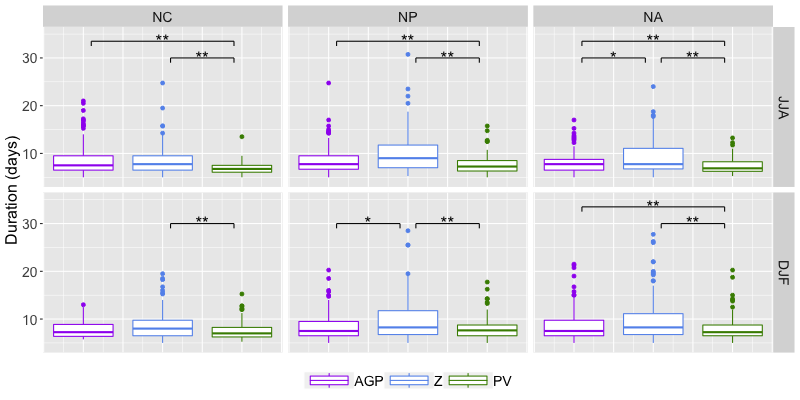
\includegraphics[width=0.75\textwidth]{fig_duration_NH.png}
    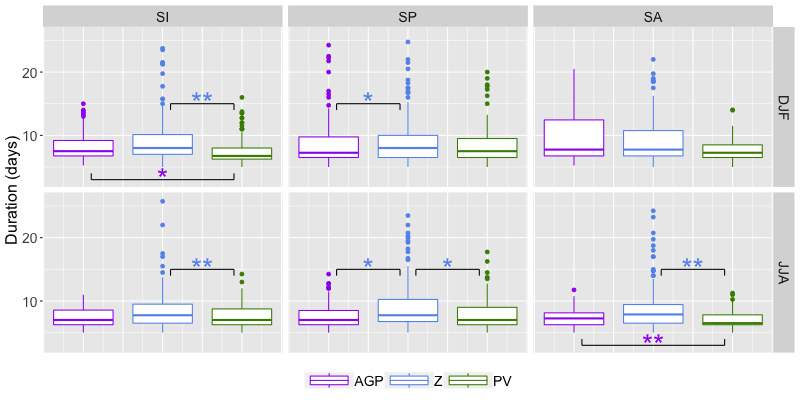
\includegraphics[width=0.75\textwidth]{fig_duration_SH.png}
    \caption{Boxplots of block duration values, in days. The brackets indicate pairs with statistically significant differences in the median values, with a ``*'' denoting $0.01<p<0.05$ and a ``**'' denoting $p<<0.01$}
    \label{duration}
\end{figure}

% \begin{table}
% \caption{Interquartile range of block duration, in days. The distribution of values is heavily skewed to the left due to the minimum 5 day duration threshold. }
% \label{duration}
% \centering

% \begin{tabular}{|c|c|l|l|l|}
% \hline
% &\multicolumn{1}{|l|}{Season} & \multicolumn{1}{c|}{AGP} & \multicolumn{1}{c|}{$Z^*$} & \multicolumn{1}{c|}{$PV^*$} \\ \hline
% \multirow{2}{*}{NH}& JJA &  \textbf{6.00} to \textbf{11.50}  &  \textit{5.75} to \textit{7.56}  &  \textit{5.75} to 8.25  \\  
% & DJF  &  \textit{5.75} to 10.50  &  \textbf{6.38} to \textbf{12.88}  &  \textit{5.75} to \textit{9.50}  \\  
%   \hline
% \multirow{2}{*}{SH}&  DJF   &  5.75 to \textit{8.75}  &  \textbf{6.25} to \textbf{10.50}  &  \textit{5.50} to \textit{8.75}  \\ 
% & \multirow{1}{*}{JJA} &  \textit{5.50} to 9.25  &  \textbf{6.75} to \textbf{14.56}  &  \textit{5.50} to \textit{8.50}  \\ 
%   \hline
% \end{tabular}

% \end{table}

\paragraph{Block duration:} These results fall within the range of previously presented values (averages of about 6-8 days), such as results from \citealt{wiedenmann_climatology_2002}, which note shorter durations in summer versus winter as well as in the SH versus the NH. The 5-day minimum threshold provides a lower bound to the range of possible 25th percentile values, but the upper bound is quite variable per method, as seen in Figure \ref{duration}. 

Overall, the $PV^*$ method had distributions of durations values with the smallest magnitudes; on average, the difference in median values between $PV^*$ and other methods was -1.34 (with $p<<0.01$). The relationship between $AGP$ and $Z^*$ is less consistent, although $Z^*$ tends to have larger extreme values. The high $AGP$ duration values, particularly in the SH, are often associated with low-latitude blocks.
%The range of duration values for $Z^*$ varied more than the other methods, with shorter-lived $Z^*$ blocks (about 6-8 days) in NH summer and the longest-lived $Z^*$ blocks (up to almost 15 days) in SH winter. The SH winter blocks detected by $Z^*$ had some of the largest overall duration values. In contrast to $Z^*$, $AGP$ blocks were overall less persistent in the SH (5.5 to 9.25 days) compared to the NH (5.75 to 11.5 days). The high $AGP$ duration values in NH summer were mainly due to low-latitude blocks. The $PV^*$ detected blocks tended towards shorter durations overall (5.5 to 9.5 days), which is partly an artifact of the size threshold, but the range of values were more consistent across seasons and hemispheres.


\begin{figure}
    \centering
    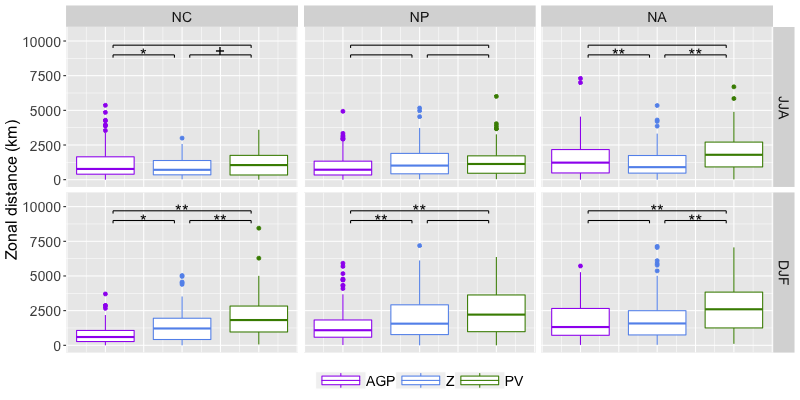
\includegraphics[width=0.75\textwidth]{fig_distance_NH.png}
    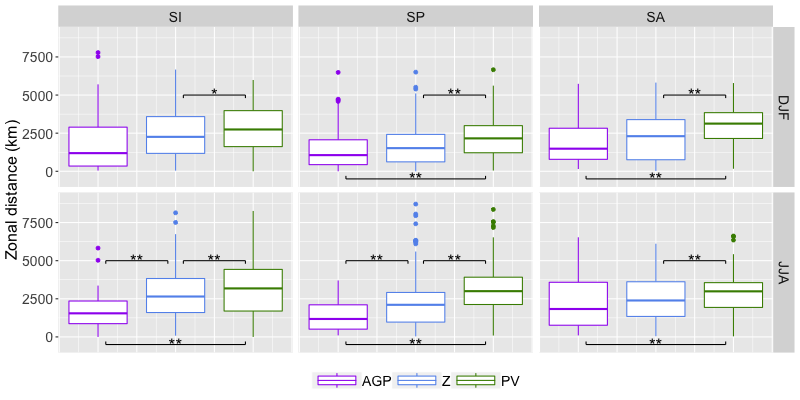
\includegraphics[width=0.75\textwidth]{fig_distance_SH.png}
    \caption{As }
    \label{dist}
\end{figure}

% \begin{table}
% \caption{Interquartile range of zonal distance traveled during block lifespan, in km. The distributions are more normal-shaped than duration distributions, although some distributions are still left-skewed.}
% \label{dist}
% \centering

% \begin{tabular}{|c|c|l|l|l|}
% \hline
% &\multicolumn{1}{|l|}{Season} & \multicolumn{1}{c|}{AGP} & \multicolumn{1}{c|}{$Z^*$} & \multicolumn{1}{c|}{$PV^*$} \\ \hline
% \multirow{2}{*}{NH}& JJA &  \textit{425.87} to \textbf{2346.63}  &  539.91 to \textit{2058.39}  &  \textbf{778.11} to 2266.02  \\
% & DJF  &  \textit{561.53} to \textit{2076.27}  &  654.26 to 2905.13  &  \textbf{954.22} to \textbf{3572.69}  \\
%   \hline
% \multirow{2}{*}{SH}&  DJF  &  \textit{510.98} to \textit{2305.94}  &  856.61 to 3211.94  &  \textbf{1379.90} to \textbf{3465.79}  \\ 
% & \multirow{1}{*}{JJA}  &  \textit{639.48} to \textit{2244.92}  &  1212.48 to 3701.14  &  \textbf{2155.11} to \textbf{4323.15}  \\ 
%   \hline
% \end{tabular}

% \end{table}
 
\paragraph{Block zonal distance traveled:} As most previous blocking studies determine blocking on a per-gridpoint basis, it is difficult to draw direct comparisons to results here. Table \ref{dist} shows that, with the exception of NH summer, $AGP$ detected regions move the least zonal distance over time; regions detected by $Z^*$ have a range of values that is up to 50\% higher than the $AGP$ values and $PV^*$ values are greater still (up to twice as large as the values of the $AGP$ interquartile ranges), despite smaller  interquartile ranges for duration. The large values in NH summer for $AGP$ can be somewhat attributed to low-latitude blocks; 38\% of $AGP$-detected regions that are equatorward of 40 degrees (113 cases out of 301) have zonal distance measurements that exceed 2000 km ($\approx$ 24 degrees longitude) over the detected block's lifetime. Some of the larger zonal distance values for $PV^*$ can be attributed to the fact that, under certain meteorological conditions (see Section \ref{shearvort}), $PV^*$ detects gridpoints that are upstream relative to those detected by the other methods, meaning that the longitude coordinate of the cluster centroid is correspondingly shifted as well.
{\color{teal}R2: I struggle to see how the fact that PV* tends to identify the blocking further upstream implies that the distance travelled will be larger according two PV* as well. Please try to explain more clearly.}
The resultant zonal distance between the start and end longitude coordinates can be hundreds of km greater than that of $Z^*$ or $AGP$, even if the three methods are tracking the same feature. Another factor involves $PV^*$-detected clusters that are embedded in regions of relatively unimpaired flow--- this is particularly prevalent at lower latitudes (see Section \ref{lowlatsec}).

\begin{figure}
    \centering
    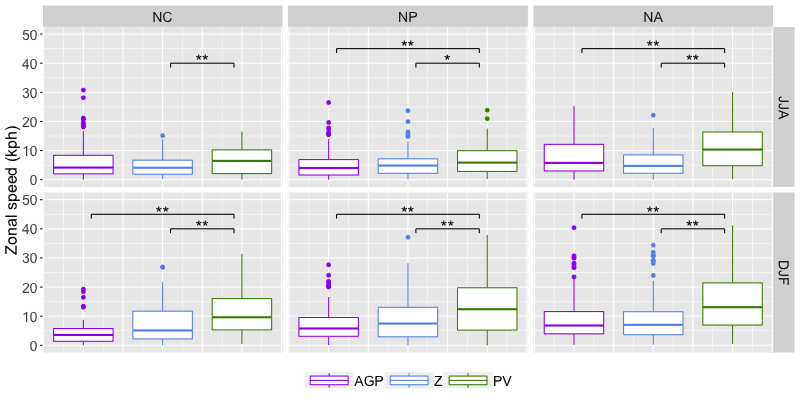
\includegraphics[width=0.75\textwidth]{fig_speed_NH.png}
        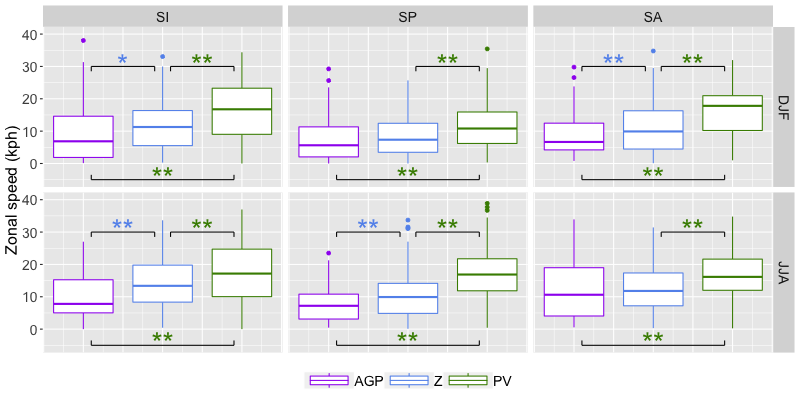
\includegraphics[width=0.75\textwidth]{fig_speed_SH.png}
    \caption{Speed distributions}
    \label{shspeed}
\end{figure}

% \begin{table}
% \caption{Interquartile range of zonal block speed (distance over duration), in km/hr. }
% \label{shspeed}
% \centering
% \begin{tabular}{|c|c|l|l|l|}
% \hline
% &\multicolumn{1}{|l|}{Season} & \multicolumn{1}{c|}{AGP} & \multicolumn{1}{c|}{$Z^*$} & \multicolumn{1}{c|}{$PV^*$} \\ \hline
% \multirow{2}{*}{NH}& JJA  &  \textit{2.11} to 10.81  &  2.83 to \textit{9.35}  &  \textbf{4.67} to \textbf{14.16}  \\  
% & DJF  &  \textit{2.86} to \textit{9.72}  &  2.97 to 12.36  &  \textbf{5.21} to \textbf{19.80}  \\ 
%   \hline
% \multirow{2}{*}{SH}& DJF&  \textit{3.14} to \textit{13.65}  &  4.25 to 15.49  &  \textbf{7.14} to \textbf{20.88}  \\
% & \multirow{1}{*}{JJA}  &  \textit{3.83} to \textit{11.70}  &  5.85 to 18.56  &  \textbf{12.99} to \textbf{24.79}  \\ 
%   \hline
% \end{tabular}
% \end{table}

\paragraph{Block zonal speed:} As with zonal distance, it is difficult to compare these results to previous studies, but \cite{sinclair_climatology_1996}, which tracks anticyclones in the SH, used a criterion of 3000 km in 5 days (or 25 km/hr) as a threshold for limiting tracking to slower-moving features. This threshold was in terms of 2D distance, rather than zonal distance as presented here, but assuming that the trajectory is mainly zonal with slight latitudinal variation, an estimate of 25 km/hr is a reasonable estimate for an upper bound. 

When the speeds, shown in Table \ref{shspeed}, are calculated (as described in Appendix \ref{stitchdesc}), the 75th percentile values of the block speeds are overall higher in the SH, which is likely associated with the stronger zonal flow in the SH. $AGP$ detected regions have the lowest speeds (mainly due to shorter zonal distances), and while $Z^*$ detected regions had larger zonal distances, they had correspondingly larger duration values as well, which leads to a range of speeds that is in between $AGP$ and $PV^*$. $PV^*$ detected regions have the largest zonal speed values due to the combination of shorter duration and longer zonal distance, particularly in the SH; the range of values are upwards of 50\% larger those from other methods, and the 25 km/hr benchmark from Sinclair is exceeded more often by $PV^*$ detected regions than the other methods. 

\begin{figure}
    \centering
    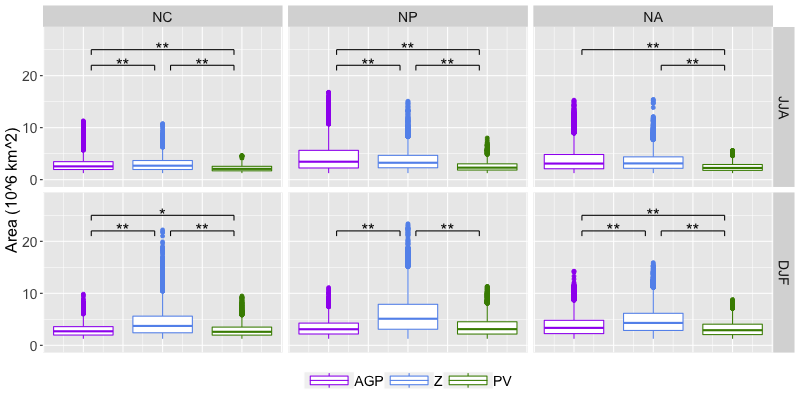
\includegraphics[width=0.75\textwidth]{fig_area_NH.png}
    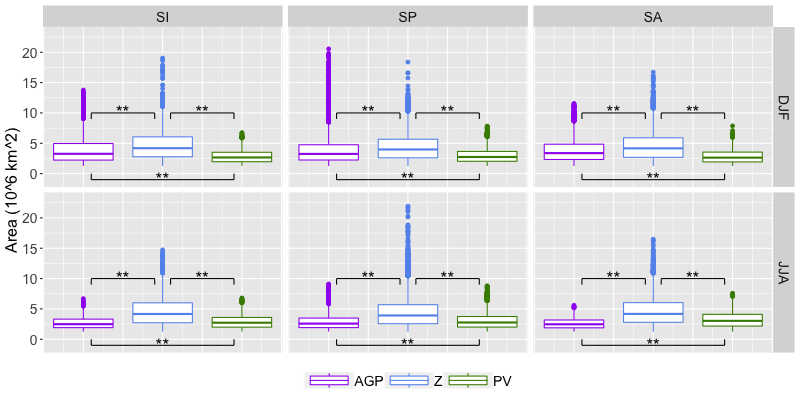
\includegraphics[width=0.75\textwidth]{fig_area_SH.png}
    \caption{Distribution of area}
    \label{size}
\end{figure} 

% \begin{table}
% \caption{Interquartile range of block size, in $ 10^6$ km$^2$.}
% \label{size}
% \centering

% \begin{tabular}{|c|c|l|l|l|}
% \hline
% &\multicolumn{1}{|l|}{Season} & \multicolumn{1}{c|}{AGP} & \multicolumn{1}{c|}{$Z^*$} & \multicolumn{1}{c|}{$PV^*$} \\ \hline
% \multirow{2}{*}{NH}& JJA &  2.35 to 3.33  &  \textbf{2.68} to \textbf{4.05}  &  \textit{2.03} to \textit{2.80}  \\  
% & DJF  &  2.76 to 3.97  &  \textbf{3.56} to \textbf{5.80}  &  \textit{2.50} to \textit{3.87}  \\ 
%   \hline
% \multirow{2}{*}{SH}& DJF&  \textit{2.37} to \textit{3.15}  &  \textbf{3.48} to \textbf{5.24}  &  2.45 to 3.37  \\ 
% &JJA &  \textit{2.36} to \textit{3.22}  &  \textbf{3.50} to \textbf{5.32}  &  2.51 to 3.59  \\
%   \hline
% \end{tabular}

% \end{table}

\paragraph{Block size:} \cite{croci-maspoli_multifaceted_2007}, which uses S04 (but without the size threshold as defined here), presents results in which detected regions in the NH range from 0.5 to $4\times 10^6$ km$^2$; Table \ref{size} summarizes the range of block sizes for each method here, and
the values for $AGP$ and $PV^*$ are in agreement with this range, while those of $Z^*$ are larger at the 75th percentile. Size is an important consideration here because it can determine whether or not a detected region is rejected due to the threshold constraint. When a blocked feature is detected by both the $PV^*$ and $Z^*$ methods, the larger $Z^*$ contour will frequently both appear earlier and persist longer than the smaller $PV^*$ contour. This is not an artifact of the threshold magnitude, as altering the magnitude of the threshold did not significantly impact the distribution of block size; $PV^*$ blocks on average will be smaller than their $Z^*$ counterparts.

\subsection{Intercomparison of blocking algorithms}\label{intercompare}

Tables \ref{pearsontabcol}-\ref{simtabcol} provide a summary of the various co-occurrence metrics between the three methods. Each section displays results for the NH and SH as separate subtables, with the summer seasons on top. Correlation and probability tables contain single numbers, as they were calculated as single quantities, but as spatial similarity was calculated for instantaneous fields at each time step containing blocking, there are a range of similarity values, presented here as interquartile ranges similar to the tables in the previous section; there are instances of fields where $S(M1,M2)>0.9$, but these are rare. 

For the correlation and probability tables,  values above (below) 0.7 (0.3) are bolded (italicized) to emphasize patterns of consistently high or low values. For the similarity table, the 25th and 75th percentile values are formatted based on the relative distributions of these values--- 25th percentile values above (below) 0.29 (0.15) are bolded (italicized), and 75th percentile values above (below) 0.54 (0.39) are bolded (italicized) to denote particularly high or low quantities relative to other values. 
{\color{teal}R2: This, too, is material for a figure or table caption.}

\begin{table}
\centering
\caption{Pearson correlation values between blocking frequencies of each region, as shown in Figure \ref{blockdens}.}
\label{pearsontabcol}
\subcaption{Northern Hemisphere}
\begin{tabular}{|l|l|l|l|l|}
\hline
 Season & Method pair & NC    & NP    & NA   \\ \hline
\multirow{3}{*}{JJA} 
   & $PV^* $ and $AGP$  & \textit{-0.21**} & -0.56** & -0.46** \\ 
   & $Z^*$ and $AGP$  & \textit{-0.19**} & -0.38** & -0.49** \\  
   & $PV^*$ and $Z^*$  & 0.51** & \textbf{0.76**} & \textbf{0.73**} \\ 
   \hline
\multirow{3}{*}{DJF}
  & $PV^*$ and $AGP$ & 0.62** & \textit{0.01} &\textit{ -0.06*} \\  
  & $Z^*$ and $AGP$  & \textit{0.26**}& \textit{-0.04+}& \textit{-0.01}  \\ 
  & $PV^*$ and $Z^*$  & 0.49** & \textbf{0.71**} & 0.45**  \\   \hline
\end{tabular}
\subcaption{Southern Hemisphere}
\begin{tabular}{|l|l|l|l|l|}
\hline
 Season & Method pair &  SI    & SP    & SA    \\ \hline

\multirow{3}{*}{DJF}
  & $PV^*$ and $AGP$  & -0.55**&-0.54** & -0.46**\\  
  & $Z^*$ and $AGP$   & -0.68**& -0.64** & -0.58**\\ 
  & $PV^*$ and $Z^*$  & \textbf{0.76**} & \textbf{0.71**} & \textbf{0.79**} \\   \hline
  
  \multirow{3}{*}{JJA} 
   & $PV^* $ and $AGP$  & -0.48** & \textit{-0.06*} & -0.59**\\ 
   & $Z^*$ and $AGP$  & -0.58** & \textit{0.09**} & {-0.53**} \\  
   & $PV^*$ and $Z^*$  & \textbf{0.70**} & {0.44**} & {0.67**} \\ 
   \hline
\end{tabular}
\end{table}

\paragraph{Pearson pattern correlation:} The results in Table \ref{pearsontabcol} highlight the clear differences in blocking frequency that will arise given the choice of an anomaly versus a total field (discussed further in Section \ref{anominst}). Since each of the methods was initially constructed using NH DJF data, it is unsurprising that these correlation values  between all variable pairs are moderate to high in this subset of data, but this does not hold for other regions. Generally, correlation values are lower in the respective summer hemispheres. $C(PV^*, Z^*)$ is strong ($>0.71$) in all regions and seasons, but (with the exception of $C(Z^*, AGP)$ in NA DJF and $C(PV^*, AGP)$ in NC DJF) correlation between $AGP$ and the anomaly methods is low (0.00-0.30) to moderate (0.31-0.70).  

\begin{table}
\centering
\caption{Probability of co-occurrence between instantaneously blocked fields.}
\label{probtabcol}
\subcaption{Northern Hemisphere}
\begin{tabular}{|l|l|l|l|l|l|l|l|l|l|}
\hline
Season & Method pair & Probability & NC    & NP    & NA      \\ \hline
\multirow{8}{*}{JJA} 
   & \multirow{2}{*}{$PV^* $ and $AGP$}&$P(PV^*|AGP)$ & \textit{0.04} & \textit{0.05} & \textit{{0.04}}  \\  
   & & $P(AGP|PV^*)$ & {0.45} & {0.46} & {0.34}  \\ 
   &&&&&\\
   & \multirow{2}{*}{$Z^*$ and $AGP$} &$P(Z^*|AGP)$    & \textit{{0.11}} & \textit{{0.18}} & \textit{{0.13} } \\  
   &&$P(AGP|Z^*)$   & {0.43} & {0.66} & {0.44} \\ 
      &&&&&\\
      & \multirow{2}{*}{$PV^*$ and $Z^*$ } &$P(PV^*|Z^*)$    & \textit{0.14}& \textit{0.29}& \textit{{0.24}} \\ 
   &&$P(Z^*|PV^*)$   & {0.48} & \textbf{{0.73}} & 0.60  \\ 
  
  \hline
  \multirow{8}{*}{DJF} 
   & \multirow{2}{*}{$PV^* $ and $AGP$}&$P(PV^*|AGP)$ & {0.38} & {0.34} &\textit{{0.21}}  \\
   & & $P(AGP|PV^*)$& \textit{{0.30}} &\textit{0.38}& {0.48}\\ 
      &&&&&\\
   & \multirow{2}{*}{$Z^*$ and $AGP$} &$P(Z^*|AGP)$ & {0.59} &0.55& {0.52} \\ 
   &&$P(AGP|Z^*)$   & \textit{{0.18} }& {0.41} & 0.53 \\ 
      &&&&&\\
      & \multirow{2}{*}{$PV^*$ and $Z^*$ } &$P(PV^*|Z^*)$    & \textit{0.24} & {0.48} & {0.31} \\
   &&$P(Z^*|PV^*)$   & {0.61} & \textbf{0.73} & \textbf{0.70}  \\   
  \hline
\end{tabular}
\subcaption{Southern Hemisphere}
\begin{tabular}{|l|l|l|l|l|l|l|l|l|l|}
\hline
  Season & Method pair & Probability & SI    & SP    & SA    \\ 
  
  \hline
  \multirow{8}{*}{DJF} 
   & \multirow{2}{*}{$PV^* $ and $AGP$}&$P(PV^*|AGP)$ & \textit{{0.01}} & \textit{{0.04} }& \textit{{0.00}} \\
   & & $P(AGP|PV^*)$ & \textit{{0.03}} & \textit{0.11}& \textit{{0.01}} \\ 
      &&&&&\\
   & \multirow{2}{*}{$Z^*$ and $AGP$} &$P(Z^*|AGP)$  & \textit{0.09} & \textit{{0.24}} & \textit{0.09} \\ 
   &&$P(AGP|Z^*)$  & \textit{{0.16} }& {{0.31} }& \textit{{0.14} }\\ 
      &&&&&\\
      & \multirow{2}{*}{$PV^*$ and $Z^*$ } &$P(PV^*|Z^*)$    & {0.40} & {0.34} & {0.34} \\
   &&$P(Z^*|PV^*)$   &\textbf{0.78} & \textbf{0.73} & \textbf{0.78} \\   
   \hline
\multirow{8}{*}{JJA} 
   & \multirow{2}{*}{$PV^* $ and $AGP$}&$P(PV^*|AGP)$ & \textit{0.13} & \textit{0.24} & \textit{0.18} \\  
   & & $P(AGP|PV^*)$  &\textit{{0.04}} & \textit{{0.20}} & \textit{{0.11}} \\ 
   &&&&&\\
   & \multirow{2}{*}{$Z^*$ and $AGP$} &$P(Z^*|AGP)$  & {0.49} & {0.66} & {0.67} \\  
   &&$P(AGP|Z^*)$    & \textit{{0.06}} & \textit{{0.18}} & \textit{{0.14}} \\ 
      &&&&&\\
      & \multirow{2}{*}{$PV^*$ and $Z^*$ } &$P(PV^*|Z^*)$    & \textit{{0.26}} & {{0.31}}& \textit{{0.28}} \\ 
   &&$P(Z^*|PV^*)$   & \textbf{{0.72}} & {\textbf{0.71}} & \textbf{0.79} \\ 
   
  \hline
\end{tabular}
\end{table}

\paragraph{Probability of co-occurrence:} Here, the interpretation of values in Table \ref{probtabcol} must take the relative quantities of each method's detected features into account. $P(Z^*|AGP)$ is high in SI and SA JJA mainly because of the small number of $AGP$ detected regions with respect to the large number of $Z^*$ detected regions, so $AGP$ is a very good predictor of $Z^*$ but the reverse is not true ($P(AGP|Z^*)$ is often less than 0.20).  Note that despite the fact that $C(PV^*,AGP)\approx C(Z^*,AGP)$ during JJA in SI  and SA, $P(PV^*|AGP)$ is not similarly high; regions detected by these two methods rarely coincide. 

When this information is combined with the correlation coefficients from the previous section, it again reinforces the point that the anomaly methods are in higher agreement than $AGP$ and the anomaly methods. Although there are two instances of high correlation between $AGP$ and the anomaly methods ($C(PV^*, AGP)$ in NC JJA and $C(Z^*, AGP)$ in NA DJF), the probability of co-occurrence between these methods is only low to moderate; this means that the averaged pattern might appear to be similar, but the methods are not simultaneously detecting the same features on a per-timestep basis. In contrast, the high values of $P(Z^*|PV^*)$, combined with the high values of $C(PV^*, Z^*)$ indicates that $PV^*$ and $Z^*$ are much more likely to detect the same features (but $PV^*$ will do so less often, given the lower blocking frequency).% {\color{blue}[MAR: another thing to add to conclusion]}

\begin{table*}
\centering

\caption{ Interquartile ranges of spatial similarity between instantaneously blocked fields.}
\label{simtabcol}
\subcaption{Northern Hemisphere}
\begin{tabular}{|l|l|l|l|l|}
\hline
  & Method pair & NC    & NP    & NA    \\ \hline
\multirow{3}{*}{JJA} 
   & $PV^* $ and $AGP$    & {0.26} to {0.46} & \textit{0.10} to \textit{0.39} & {0.20} to \textit{0.45}  \\  
   & $Z^*$ and $AGP$   & \textbf{0.36} to \textbf{0.58} & {0.20} to {0.43} & {0.25} to {0.52}  \\   
   & $PV^*$ and $Z^*$   & \textbf{0.34} to \textbf{0.56} & \textbf{0.32} to \textbf{0.54} & \textbf{0.31} to \textbf{0.55}  \\ 
   \hline
\multirow{3}{*}{DJF}
  & $PV^*$ and $AGP$ & \textbf{0.29} to \textbf{0.54} & {0.22} to {0.45} & \textit{0.16} to {0.44} \\   
  & $Z^*$ and $AGP$ & \textbf{0.34} to \textbf{0.56} & {0.18} to {0.42} & 0.25 to {0.50} \\ 
  & $PV^*$ and $Z^*$   & {0.28} to \textbf{0.56} & {0.24} to {0.51} & {0.28} to \textbf{0.54} \\  
  \hline
\end{tabular}
\subcaption{Southern Hemisphere}
\begin{tabular}{|l|l|l|l|l|}
\hline
  & Method pair & SI    & SP    & SA      \\ \hline

\multirow{3}{*}{DJF}
  & $PV^*$ and $AGP$  & \textit{0.04} to \textit{0.28} & \textit{0.09} to \textit{0.38} & \textit{0.06} to \textit{0.13} \\   
  & $Z^*$ and $AGP$ & \textit{0.14} to \textit{0.27} & {0.20} to \textit{0.38} & {0.23} to \textit{0.29} \\ 
  & $PV^*$ and $Z^*$  & \textbf{0.36} to \textbf{0.59} & \textbf{0.34} to \textbf{0.61} & \textbf{0.38} to \textbf{0.59} \\  
  \hline
  \multirow{3}{*}{JJA} 
   & $PV^* $ and $AGP$    & \textit{0.15} to \textit{0.30} & \textit{0.11} to \textit{0.34} & \textit{0.11} to \textit{0.37} \\  
   & $Z^*$ and $AGP$   & {0.21} to \textit{0.38} & {0.18} to {0.40} & {0.20} to \textit{0.31} \\   
   & $PV^*$ and $Z^*$   & {0.26} to {0.51} & {0.22} to {0.48} & \textbf{0.29} to \textbf{0.56} \\ 
  \hline
\end{tabular}

\end{table*}


\paragraph{Spatial similarity:} The third measure of agreement between methods, spatial similarity, is highly influenced by the size and location of detected regions relative to one another. Note that the largest 75th percentile value is 0.61, which is unsurprising given the differences in detected block size between methods even if the same feature is detected.   The results in Table \ref{simtabcol} provide additional insight to the results from the previous two sections. While $PV^*$ and $Z^*$ again have some of the highest values for similarity relative to other combinations of methods, $S(PV^*,Z^*)$ rarely exceeds 0.6, and more often in the respective summer hemispheres when the $Z^*$ blocks are smaller. Additionally, $S(PV^*,AGP)<S(Z^*,AGP)$ in most instances; this is sometimes due to the relative sizes of the detected contours, but the $PV^*$ detected contour is also sometimes shifted with respect to the $Z500$-based methods (example in Section \ref{shearvort}).% {\color{blue}[MAR: another thing to add to conclusion]}

\subsection{Case study: The Ridiculously Resilient Ridge}\label{rrrsec}

{\color{teal}R2: This is at the discretion of the authors, but could it be advantageous to discuss the case study at the start of the paper, thereby introducing many concepts, and making the paper easier to understand overall?}

To highlight the importance of selecting a method that will ``correctly'' identify desired features, we present an example of a persistent and pronounced ridge pattern that repeatedly appeared off the western coast of North America in late 2013, then reoccurred during the winters of 2014-2015 and 2015-2016. This feature, dubbed the ``Ridiculously Resilient Ridge'' (or RRR for short) by \cite{swain_extraordinary_2014}, was responsible for redirecting moisture-heavy air northwards during the winter months. Because California receives the bulk of its precipitation from December to March, the RRR was a key player in the drought that devastated the state for almost 6 years. 

\begin{table*}
\caption{Pattern correlation, probability of co-occurrence, and spatial similarity for RRR data (DJF, December 2012-February 2016). }\label{RRRtable}
\centering
\begin{tabular}{|l|ccc|}
\hline
Method pair & Correlation & Probability & Similarity \\
\hline
\multirow{2}{*}{$PV^*$ and $AGP$} & \multirow{2}{*}{0.38} & $P(PV^*|AGP)$: 0.44 & \multirow{2}{*}{0.21 to 0.51} \\
& & $P(AGP | PV^*)$: \textit{0.24 }& \\
& & & \\
\multirow{2}{*}{$Z^*$ and $AGP$} & \multirow{2}{*}{0.41} & $P(Z^*|AGP)$: \textbf{0.76} & \multirow{2}{*}{0.16 to 0.40} \\
& & $P(AGP | Z^*)$: \textit{0.19} & \\
& & & \\
\multirow{2}{*}{$PV^*$ and $Z^*$} & \multirow{2}{*}{0.48} & $P(PV^*|Z^*)$: 0.42 & \multirow{2}{*}{0.26 to 0.48} \\
& & $P(Z^* | PV^*)$: \textbf{0.89} &  \\
\hline
\end{tabular}
\end{table*}



Figure \ref{RRRFreq} shows the frequency of detected blocking in NP DJF from December 2012 to February 2016, and Table \ref{RRRtable} provides the corresponding agreement metrics. Out of the three methods, the one that most closely coincides with the location of the RRR---in terms of a blocking maximum centered off of the West Coast---is the $Z^*$ method. The $PV^*$ method displays the previously noted inclination towards contours that co-locate with $Z^*$ contours ($P(Z^*|PV^*)=0.89$), but the maximum is positioned further northwards and there is only a modest correlation of $C(PV^*, Z^*)=0.48$. Due to the $PV^*$ method's propensity to focus on the ridge peak, $PV^*$ also picks up about half as many instances of ridging (averaged blocking frequency of 9\%, $\sim$8.28 days per season at its maximum over Alaska) as $Z^*$ (averaged blocking 18\%, $\sim$16.56 days per season in the location of the $PV^*$ blocking frequency maximum). The $AGP$ method has an averaged blocking frequency that about equals $PV^*$ over Alaska, and a high probability of co-occurrence with $Z^*$ ($P(Z^*|AGP)=0.76$), but its maximum during this time is positioned over the Western Pacific, indicating that it is less likely to identify the particular feature that we are interested in identifying here. 

The reason for this difference in the average blocking patterns with respect to the RRR becomes apparent in Figure \ref{RRRpanel}. In each of these examples, the blocks detected by the $AGP$, $Z^*$ and $PV^*$ methods are outlined in purple, blue, and green solid lines, respectively, and the thin contours depict 500 hPa geopotential height in 50 m increments. Many times, the ridge that appears off the North American west coast has a north/south oriented ridge axis with little to no horizontal tilt; therefore, the $GHGS$ criterion of the $AGP$ method is not fulfilled, as will be discussed in Section \ref{anominst}. The blocking pattern seen on December 7th, 2013 (Figure \ref{RRRpanel}d) is one of the exceptions, due to both the slight westward tilt (with increasing latitude) of  the ridge axis and the local Z500 maximum at 220E, both of which satisfy $GHGS>0$. However, even in this example, where all three methods detected the feature, they defined the extent of the block differently; comparing the three methods, $S(PV^*,Z^*)=0.53$, $S(PV^*,AGP)=0.36$, and $S(Z^*,AGP)=0.22$ If these detection algorithms were to be used in some sort of predictive capacity, the $Z^*$ method would pick up RRR-like features every time they occurred, but detect many additional features as well. The $PV^*$ method would detect some of the same features as $Z^*$, but it would also miss some instances, as in Figure \ref{RRRpanel}b, and would not define the extent of the block in the same way. Like $PV^*$, the $AGP$ method would also miss some of these features, as well as identifying others that are not relevant here. 

If the goal is to detect a ridge configuration similar to that of the RRR, then the results suggest that of the three algorithms discussed in this paper, the $Z^*$ algorithm is the most reliable method to find the ridge, with $PV^*$ acting as a more conservative substitute method. The algorithm design of $AGP$ does not deal well with the particular block shape that appears frequently during this time; therefore, the use of $AGP$ is not ideal for performing an analysis on future trends in blocking specific to the western United States. 


\section{Meteorological drivers of differences between blocking algorithms}\label{influences}

The various metrics displayed in Section \ref{results} show that all three of the methods have widely varying definitions of blocks, from the block's physical characteristics to whether or not a block is actually present at a particular point in time. The RRR case study, in particular, highlights the importance of considering the nature of the region's flow field and prevailing block type when selecting the appropriate detection method. A few meteorological factors that influence the differences between block detection methods are discussed next.


\subsection{Anomaly versus total field Z500-based methods}\label{anominst}

In Section \ref{intercompare}, the magnitudes of the agreement metrics show that there is a clear distinction between circumstances when blocks are detected by $AGP$, a method based on the total $Z500$ field, as opposed to the other two methods that are based on anomalies with respect to the LTDM. We limit the discussion here to the two methods that are based on $Z500$ in order to reduce other sources of variability.

Both $Z^*$ and $AGP$ were created with the purpose of detecting high values of $Z500$, but $AGP$ has no reference to the mean climatology; instead, it requires a significant change in $Z500$ over a latitude range (30 degrees) that equates to more than half of each study region's latitude range (50 degrees). The difference in block detection is most evident in the SH, where there is a much stronger zonal flow component than in the NH. This stronger zonal flow implies that the requirements of the $AGP$ method are fulfilled far less often in the SH, since there is not sufficient distortion of the flow field; $AGP$-detected blocks in the SH are often co-located with lows (dipole or omega blocks) or have a tilt in their north-south axis, since this guarantees that there is a sufficiently large $Z500$ gradient. In contrast, $Z^*$ is much less discriminating; it detects a high number of blocks in the SH because the $\overline{Z500}$ field has a strong meridional gradient in addition to its mainly zonal flow, meaning that even fairly shallow ridges in the $Z500$ field are more likely to satisfy $Z^*$ anomaly thresholds. 

These points are illustrated in Figure \ref{zgdiff}, which shows a snapshot of an omega block in SP on May 5th 18Z 1998 (left) and 12 hours later (right). At the earlier time, the two anomaly methods produce clusters that are centered over the ridge ($S(PV^*, Z^*)=0.78$), but the $AGP$ method only picks out an area centered polewards of the lower geopotential heights to the east of the ridge (before the size constraint was applied, there was also a detected region in the vicinity of 190E,65S); $S(PV^*, AGP)=0.24$ and $S(Z^*, AGP)=0.26$. Later, the intensification of the high in the 60-70S latitudes produces the necessary height gradient to satisfy the criteria for $AGP$; $S(PV^*, AGP)=0.46$ and $S(Z^*, AGP)=0.58$. 

\subsection{$PV^*$ links to shear and vorticity}\label{shearvort}

The $PV^*$ method picks out regions with PV that are highly anomalous with respect to the climatological mean in the upper troposphere. Most often, these regions are areas with particularly pronounced anticyclonic circulation in the $Z500$ field, such as dipoles or omega blocks. The $PV^*$ method tends to detect blocks at higher latitudes than the other two methods during each respective hemisphere's summer, and a more varied winter distribution; this pattern corresponds roughly to the location of the 500 hPa jet, which shifts from polewards of 45 degrees latitude in summer to 40 degrees latitude and below in the wintertime. 

{\color{teal}R2:I am not following what is meant by ", and a more varied winter distribution, …" and all the way to the end of the paragraph.}

Since anomalous vorticity and anomalous highs are linked, the two anomaly methods are often very similar in terms of the location of the detected block, even if the size of the detected cluster of grid points is not always the same. However, the EPV field can be influenced by phenomena such as vertical shear (first two terms in Equation \ref{pveq}) or locally strong winds; it is a factor to consider in flow that does not have the necessary meridional component to satisfy points 1 and 2 of the AMS definition of blocking. For example, a jet streak embedded in otherwise zonal flow will lead to mistaken identification of a region as blocked even though there is neither persistent obstruction nor pronounced meridional flow; the distribution of $PV^*$ zonal distances values has larger magnitudes than the other two methods (especially in the SH) because these detected regions are less stationary. 

Figure \ref{pvdiff} demonstrates a case in which a $PV^*$ detected cluster is shifted relative to clusters detected by the other two methods, despite all of the methods identifying the same block. The 4-panel figure shows an omega block that is detected by all three methods in 1989 NA SON; however, in Figure \ref{pvdiff}a, the $Z^*$ and $AGP$ contours both center on the high that is the top half of the block ($S(Z^*, AGP)=0.54$), while the $PV^*$ contour is shifted westwards ($S(PV^*, Z^*)=0.32$, $S(PV^*, AGP)=0.20$). Daily composites of the corresponding total wind (Figure \ref{windfield}) show that, on September 28th 6Z, 1989 (Figure \ref{windfield}a), there was a jet streak on the upstream side of the high pressure feature which is being detected by the three algorithms. The vorticity ($-g\zeta \frac{\partial \theta}{\partial p}$ in Equation \ref{pveq}) associated with the anticyclonic curvature of the high is strongly negative at this time, and further enhanced by vertical shear in the jet streak region. The combination of these factors leads to the westward extension of the $PV^*$ detected cluster relative to the other two clusters. As time progresses (Figures \ref{windfield}b and \ref{windfield}c), a portion of the  $PV^*$ detected contour continues to track that jet streak, which coincides with strongly negative vorticity, until it reaches a higher latitude. At that higher latitude (Figure \ref{windfield}d) $\overline{PV}$ is larger and there is positive vorticity associated with the low, meaning that the anomaly is no longer exceeding the threshold. Hence, the $PV^*$ cluster separates from the jet streak and is in better agreement with the other two methods ($S(PV^*, Z^*)=0.55$, $S(PV^*, AGP)=0.54$). 

\subsection{Low-latitude blocking and flow impairment}\label{lowlatsec}

Low-latitude blocking with respect to NH summer and the $AGP$ method is discussed in \citep{davini_bidimensional_2012};
{\color{teal}R2: "this paper" - avoid the pronoun here, because it is actually unclear which paper this refers to - Davini et al. or Pinheiro et al.}
{\color{blue}\sout{the authors of this paper question}This paper questions} whether these features are correctly characterized as blocks, since they are linked to poleward displacement of subtropical easterlies and are less intense and persistent than those at higher latitudes. Low-latitude blocking is present in all three methods: the $AGP$ method has relative maxima in the averaged blocking patterns in the respective summer hemispheres, and the $PV^*$ and $Z^*$ methods find low-latitude blocks in the respective winter hemispheres, particularly in NP DJF. Many of these low-latitude features are nearly stationary (block speed averages 2-12 km/hr in both hemispheres) and persistent (block duration averages 6-12 days in both hemispheres). However, they do not always impair the zonal flow as required by the first point in the AMS definition.

Figure \ref{lowlatjja} shows an example of one of the more stationary low-latitude $AGP$ blocks in JJA, a persistent ridge over the eastern United States in 1984 that lasted from June 8th 12Z to June 17th 0Z and had an average zonal speed of 3.84 km/hr over 8.5 days. Averaged over the detected block's lifespan, the 850 hPa temperature anomaly ($T_a$) in the vicinity of the detected block is approximately +2K,the 500 hPa meridional wind anomaly ($v_a$) is approximately $\pm6$ m/s on either side of the block, and the 500 hPa zonal wind anomaly ($u_a$) is up to -12 m/s in the blocked flow region (see Figure \ref{avgjja}). 

In contrast, Figure \ref{lowlatdjf} shows a low-latitude case in NP DJF in which two methods identify a block in the midst of flow that is not sufficiently diverted or slowed. This example shows January 5th 0Z to January 11th 0Z, 2006, where both the $Z^*$ and $PV^*$ methods detected a relatively shallow ridge that evolves into mostly zonal flow by the end of the detected block's lifespan. The $PV^*$ detected region has an average zonal speed of 6.98 km/hr over 6 days and the $Z^*$ detected region has an average zonal speed of 10.91 over 11.5 days (the difference is mainly due to the longer lifespan of the $Z^*$ detected region). $u_a$ is -16 m/s in bottom half of the blocked flow region outlined in Figure \ref{avgdjf}, but northwards of 35N, $u_a$ has a maximum magnitude of 20 m/s. $v_a$ is $\pm 10$ m/s on either side of the block and $T_a$ is +5K within the blocked region, both of which are larger anomalies than the JJA case. However, one must always approach anomalies with caution; the Z500 field in Figure \ref{lowlatdjf} does not indicate that the zonal flow has been reduced at later times. Indeed, composites of the total wind fields in Figure \ref{totwind} show that while the JJA case has reduced wind speeds (maximum 5 m/s in the blocked region, compared to 20 m/s outside the impaired region), the DJF case has wind speeds of up to 35 m/s in the northern portion of the ``blocked'' region, which also coincides with the positive $u_a$ value in the northern half of the outlined region in Figure \ref{avgdjf}. In the case of $Z^*$, this mistaken identification can be attributed to a fairly shallow ridge in an area with a strong meridional gradient (as in Section \ref{anominst}). In the case of $PV^*$, vorticity values were only slightly negative or close to 0, but when considering $VPV$ compared to $\overline{VPV}$, sufficiently anomalous for $VPV^*$ to surpass the local threshold value of 1.2 PVU.

These examples suggest that not all low-latitude blocking should be discounted, at least according to certain metrics; thus, applying blocking algorithms over a range of latitudes rather than a single central latitude will produce a more complete climatology of blocking hotspots. A number of detected low-latitude blocks will fail to meet the AMS blocking criteria, as seen in the second example. However, algorithm ``failures'' are not unique to the lower latitudes; therefore, rather than restricting analysis to a limited range of latitudes, future research should consider algorithm limitations, which have been mentioned in previous sections, and make use of additional diagnostic metrics to filter out non-blocked flow.

\section{Conclusions}\label{concsec}

\begin{table}
\caption{Summary of notable  blocking frequency distribution and block characteristics.} \label{featuretable}
%\resizebox{0.98\textwidth}{!}{
\begin{tabular}[t]{|L{0.18\textwidth}|L{0.27\textwidth}|L{0.27\textwidth}|L{0.27\textwidth}|}\hline
 &$AGP$& $Z^*$ & $PV^*$\\
\hline
\multirow{2}{0.18\textwidth}{\textbf{Flow field sensitivity}}
& Equatorward low
& Strong high
& Strong curvature \\
& Strong poleward $Z500$ gradient
& Strong $Z500$ meridional gradient
& Strong winds, vertical shear\\
&&&\\
\textbf{Favored block types }
& Omega block or ridge with meridional axis tilt
& All kinds (with sufficiently large $Z500^*$)
& All kinds (with sufficiently large $VPV^*$) \\
& Cutoff low
& 
& \\
&&&\\
\textbf{Spatial distribution of frequency }
& NH: Higher latitudes (exception of JJA low-latitude blocking), Atlantic Ocean basin (and some East Pacific)
& blocks detected over full range of study regions
& Higher latitudes in summer seasons, wider range of latitudes in winter seasons\\
& SH: blocking mostly in SP
&
& \\
&&&\\
\textbf{Location (frequency)  of maximum }
& NH JJA equatorwards of 45 degrees (25\%)
& NP DJF equatorwards of 45 degrees (21\%)
& NP DJF equatorwards of 45 degrees (12\%) \\
&&&\\
\textbf{Notable features}
& Less similar to other two methods
& Highest frequency of SH blocking
& Lowest overall frequency magnitude between methods\\
&&&\\
\textbf{Duration }
& Longest between methods in NH summer ($6-11.5$ days), $\approx 5.5-10.5$ days otherwise
& Shortest between methods in NH summer ($5.5-7.5$ days), longest otherwise ($\approx 6-14.5$ days)
& Shortest overall between methods (5.5-9.5 days) \\
&&&\\
\textbf{Zonal distance traveled}
& Shortest overall between methods ($\approx 400-2400$ km)
& $\approx 500-3700$ km
& Longest overall between methods ($\approx 800-4300$ km)\\
&&&\\
\textbf{Zonal speed}
& Slowest overall between methods ($\approx 2-13$ km/hr)
& $\approx 3-18.5$ km/hr
& Fastest overall betweem methods ($\approx4.5-25$ km/hr)\\
&&&\\
\textbf{Size}
& Smallest between methods in SH ($2.4-3.2\times 10^6$ km$^2$), $2.4-4\times 10^6$ km$^2$ in NH
& Largest overall ($2.6-5.8\times 10^6$ km$^2$)
& Smallest between methods in NH ($2-3.8\times 10^6$ km$^2$), $2.5-3.6\times 10^6$ km$^2$ in SH\\
\hline
\end{tabular}
%}
\end{table}

\begin{table}
\caption{Summary of notable observations for intercomparison of objective detection methods.} \label{inttable}
%\resizebox{0.98\textwidth}{!}{
\begin{tabular}[t]{|L{0.18\textwidth}|L{0.27\textwidth}|L{0.27\textwidth}|L{0.27\textwidth}|}\hline
 &$PV^*$ and $AGP$& $Z^*$ and $AGP$ & $PV^*$ and $Z^*$\\
\hline
\textbf{Correlation }
& Low (NP and NA summer) to moderate (NC summer, all winter); high NC winter
& Low (SA and SI summer)  to moderate (NH, SP summer, SH winter); high NP DJF
& High correlation for all regions and seasons (despite different frequency magnitudes)\\
&&&\\
\textbf{Probability of co-occurrence}
& Low to moderate for both $P(PV^*|AGP)$ and $P(AGP|PV^*)$
& Moderate to high $P(Z^*|AGP)$ when many $Z^*$, low otherwise
& Moderate to high $P(Z^*|PV^*)$ in all regions\\
&&&\\
\textbf{Spatial similarity}
& Lowest ranges of similarity values compared to other method pairs
& $S(Z^*,AGP)>S(PV^*,AGP)$
&Highest range of similarity values compared to other method pairs in almost all regions and seasons\\

\hline
\end{tabular}
%}
\end{table}

This study examines the blocking climatologies of six regions over summer and winter seasons, and highlights some of the block characteristics from three detection methods, which can be seen in Table \ref{featuretable}. Maximum blocking frequency ranged from 12\% ($PV^*$) to 25\% ($AGP$), with the locations of maximum blocking differing between $AGP$ and the anomaly methods. Some methods, such as the $PV^*$ method, are quite conservative, showing comparatively smaller frequencies and detecting smaller clusters; while others, such as the $Z^*$ method, are less discriminating with respect to regions that are defined as blocked, displaying both higher frequencies and larger clusters. 

The intercomparison of the results, as summarized in Table \ref{inttable}, raises some points that should be considered in future blocking studies that use objective detection algorithms.   Previous blocking studies often present averaged results, rather than examining them on a per-block basis, but high averaged pattern correlation does not imply that two methods will simultaneously detect the same features; furthermore, even when all three methods detect the same feature, they do not necessarily define the block using the same cluster of gridpoints. The $AGP$ and anomaly methods had a much lower degree of agreement than that between $PV^*$ and $Z^*$, in both the averaged and instantaneous sense. However, even the agreement between $PV^*$ and $Z^*$ is affected by the relative sizes and placement of the detected clusters, and the RRR case study demostrates that the block configuration is an important element to ``successful'' detection of a block. This has implications to studies which attempt to link blocking to extreme weather, because attempts to correlate the location of the block with the location of extremes will produce different results based on the chosen algorithm. 

The ideal blocking detection algorithm (one that detects all features that satisfy the AMS definition) likely requires elements from multiple detection algorithms (such as \cite{dunn-sigouin_evaluation_2012} or \cite{barriopedro_application_2010}, which combine elements of TM90 and DG83), as well as measurements of metrics such as block intensity (developed by \citealt{wiedenmann_climatology_2002}) and flow diversion. Additionally, such an algorithm would need to take seasonal and regional differences of the flow field into account.   The results show that there remains a significant discrepancy between published methods with regards to how the AMS definition is interpreted, from the calculated blocking frequencies to the average size and speed of the detected features. Many of the detected regions are persistent in the sense that they are relatively nonstationary for at least 5 days, but the resultant changes to wind speed and temperature are inconsistent. Blocks are a continuum of forms, rather than clearly delineated idealized shapes; and each method is optimized for detecting certain kinds of features under certain kinds of climatological conditions. 

This study has produced a comprehensive summary of the factors that influence block detection by three different algorithms, and noted the relative strengths and weaknesses of these methods.  Additionally, we have outlined a number of metrics for both assessing individual methods and comparing the results between methods. As part of this study, a publicly-available software package has been developed that can be used for automated block detection and tracking in arbitrary global climate datasets.
{\color{teal}R2: Please include a pointer to the software and its documentation here.}
Objective algorithms show promise for analyzing current and future trends, given their applicability to extremely large volumes of high resolution data. Using results from historical models can provide a confidence bound on anticipated changes in blocking characteristics in future climate simulations, but careful consideration of algorithm biases should be factored into the analysis.

% BibTeX users please use one of
%\bibliographystyle{spbasic}      % basic style, author-year citations
%\bibliographystyle{spmpsci}      % mathematics and physical sciences
%\bibliographystyle{spphys}       % APS-like style for physics

\bibliography{Paper1_w.bib}

\begin{appendices}

\section{Vertically averaged potential vorticity}\label{vpveq}

In its simplest form, Ertel's potential vorticity (EPV) is written as

\begin{equation}
EPV = \frac{\zeta_a\cdot \nabla \theta}{\rho}\label{epv}
\end{equation}

\noindent
Assuming hydrostatic balance in order to eliminate density, (\ref{epv}) can be written as 

\begin{equation}
  EPV=g\left(\frac{1}{r\cos\phi}\frac{\partial v}{\partial p}\frac{\partial \theta}{\partial \lambda}-\frac{1}{r}\frac{\partial u}{\partial p}\frac{\partial \theta}{\partial \phi}-(\zeta+f)\frac{\partial \theta}{\partial p}\right)\label{pveq}
\end{equation}

\noindent
in which $g$ is the gravitational constant, $r$ is the Earth's radius, $u$ and $v$ are the zonal and meridional wind components respectively, $\theta$ is potential temperature, and $\zeta + f$ is absolute vorticity.


The form presented in Equation \ref{pveq} is in spherical coordinates ($\lambda, \phi$) in the horizontal direction and pressure level coordinates ($p$) in the vertical. 


For S04, the EPV is vertically averaged over the 150-500 hPa layer using the integral method, 
\begin{equation}VPV=\frac{1}{(p_1-p_2)}\int_{p_1}^{p_2} EPV(p) dp\end{equation}

\noindent
where $p_1=1.5\times 10^4$ Pa and $p_2=5\times 10^4$ Pa, respectively.
\section{Blocking Events and the StitchBlobs Software}\label{stitchdesc}

All of code used to produce these results are included in the TempestExtremes software package \citep{ullrich_tempestextremes:_2017}, a C++-based framework for feature detection and quantification (available at \texttt{https://github.com/ClimateGlobalChange/tempestextremes}). The algorithm for the $AGP$ method is contained to a single binary, \texttt{BlockingGHG}, while the calculations for $PV^*$ and $Z^*$ involve a multi-step process which is outlined in Section \ref{modanom} and Figure \ref{stitchfig}. 


The \texttt{StitchBlobs} binary takes the outputs from the desired algorithm and applies the spatiotemporal constraints, and the corresponding \texttt{BlobStats} binary produced summary text files which include per-feature information about:
\begin{itemize}
\item Minimum/maximum latitude and longitude coordinates
\item coordinates of block centroid
\item block area (in terms of fractional area)
\end{itemize}

This information is mainly used in Section \ref{blockingmetrics}, and the quantities are defined as follows:

\begin{itemize}
\item \textit{Block duration:} the number of time steps for which block is present, multiplied by the time resolution.
\item \textit{Block zonal distance:} The difference between the start and end longitudes, converted to km.
\item \textit{Block zonal speed:} Distance divided by duration.
\item \textit{Block size:} Fractional area multiplied by the Earth's surface area, $SA = 4\pi (6371)^2$ km$^2$
\end{itemize}

A previous attempt to average speeds calculated over each 6 hour period was discarded because the center coordinate would occasionally ``jump'' in between subsequent time steps due to a change in the detected block's size---usually caused by merging of distinct features--- and a subsequent shift in the centroid. This ``jump'' led to large zonal distance values and, consequently, artificially high block speed values. The method used here (distance from start to finish, divided by duration) has its own drawbacks, as two methods tracking the same block might yield different block speed measurements if the duration and distance measurements differ between the two methods.

\section{Probability of co-occurrence calculation}\label{probcalc}

Co-occurrence is defined as the overlap between blocked regions detected by two or more different methods, which corresponds to a region of $C_k=2$ in similarity calculations. We quantified co-occurrence by counting the time steps in which there was overlap ($n[M1\cap  M2]$) during the similarity calculations as well as the number of blocks for each of the methods ($n[M1]$, $n[M2]$, etc), then finding $\min(n[M1],n[M2],n[M1\cap M2])$ per time step.

The probability of co-occurrence is defined as 

\begin{equation}
P(M1|M2) = \frac{P(M1\cap M2)}{P(M2)}
\end{equation} which translates to the number of times that blocks detected by methods M1 and M2 overlap over the number of times that blocks detected by method M2 occur.


\section{Spatial similarity calculation}\label{simcalc}

This method is similar in concept to the Jaccard index \citep{jaccard_nouvelles_1908}, also known as intersection over union:

\begin{equation}
J(A,B) = \frac{A\cap B}{A\cup B} = \frac{A\cap B}{A+B-A\cap B}
\end{equation}

\noindent
where $A\cap B$ are the common points between $A$ and $B$ and $A\cup B$ are the sum total of points in $A$ and $B$, minus the number of common points. In this instance, spatial similarity calculations are performed on two fields $M1$ and $M2$, consisting of regularly spaced grid points whose values are either 1 (block) or 0 (not a block) according to the corresponding objective detection method. 

However, there are two points to consider in these calculations:
\begin{enumerate}
\item We only wish to count common presence, not common absence (in order to quantify the amount of agreement when two methods detect a block).
\item A simple count of commonly blocked gridpoints between two methods will overemphasize spatial agreement at higher latitudes, since the meridians converge at the poles and the actual distance between gridpoints is shorter.
\end{enumerate}

To address point 1, the two fields are summed together ($F=M1+M2$), where gridpoints have values of  0 (no detection), 1 (one method detects blocking), or 2 (both methods detect blocking); only nonzero gridpoints in $F$ are considered. 

For each cluster $C_k$ of contigous nonzero gridpoints on $F$

\begin{equation}
S(C_k) = \frac{\sum\limits_{n=1}^{P_k}\left(v_n-1\right)\cos(\phi)_n}{\sum\limits_{n=1}^{P_k}cos(\phi)_n}
\end{equation}

where $P_k$ is the number of points in $C_k$, $v_n$ is the value of the gridpoint (either 1 or 2), and $cos(\phi)_n$ is the cosine of that gridpoint's latitude value. 

Summing the cosine latitude values of gridpoints, rather than the number of points in $C_k$, addresses point 2, as $\cos(\phi)_n$ is smaller at higher latitudes (thus approximating the smaller area between gridpoints). The numerator is essentially the intersection of blocked points ($M1\cap M2$); the sum will only include $\cos(\phi)_n$ where $v_n=2$ (since $v_n=1$ means that $\cos(\phi)_n$ is multiplied by 0). The denominator is the union ($M1\cup M2$), where all $\cos(\phi)_n$ are included in the sum. 

\end{appendices}




\pagebreak

\begin{figure*}
\centering
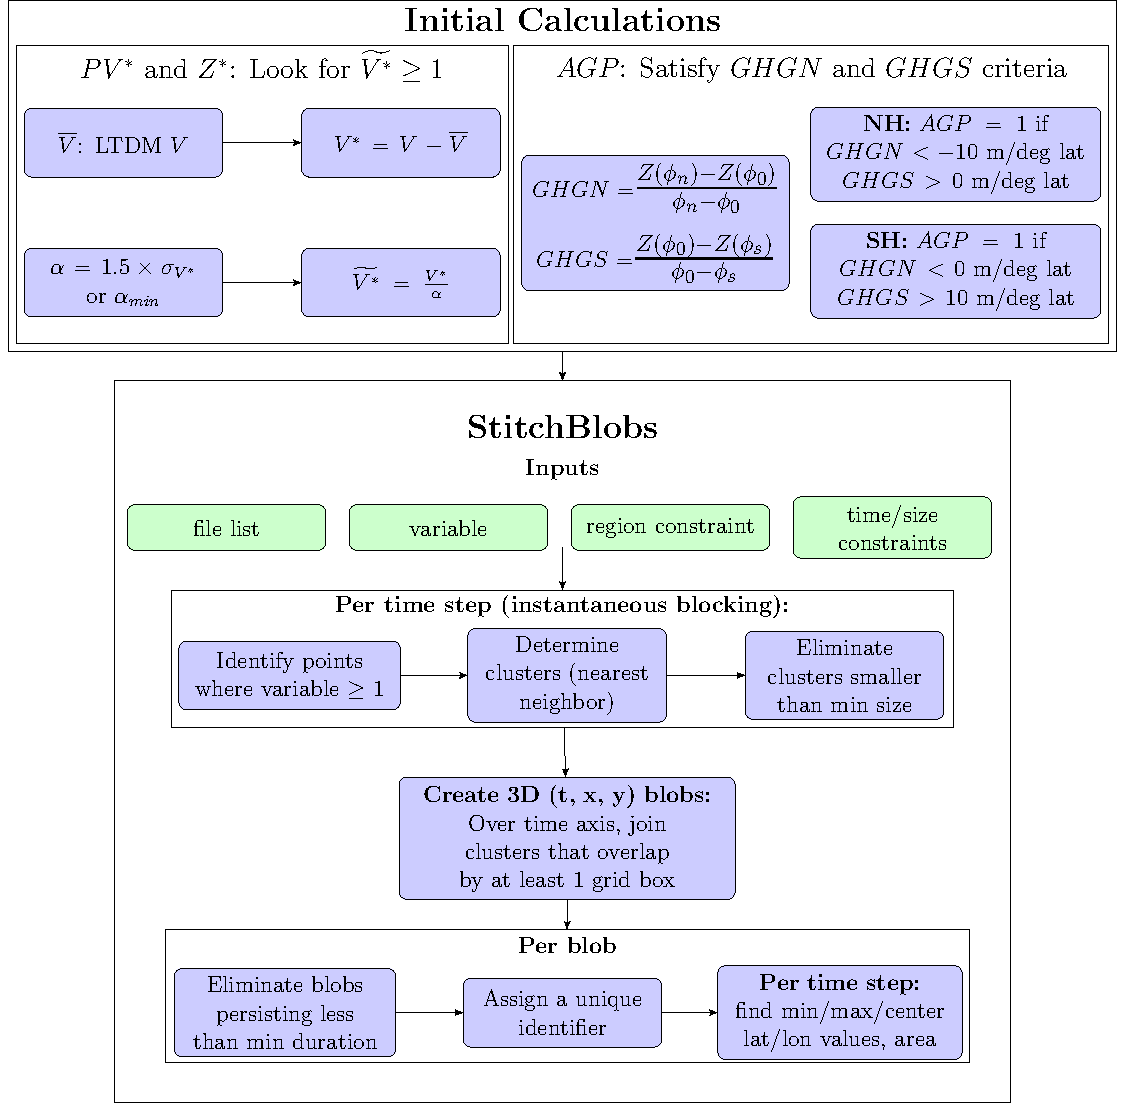
\includegraphics[width=0.75\textwidth]{fig1.pdf}
\caption{Schematic of workflow for blocking calculations using StitchBlobs}\label{stitchfig}
\end{figure*}

\begin{figure*}
\centering
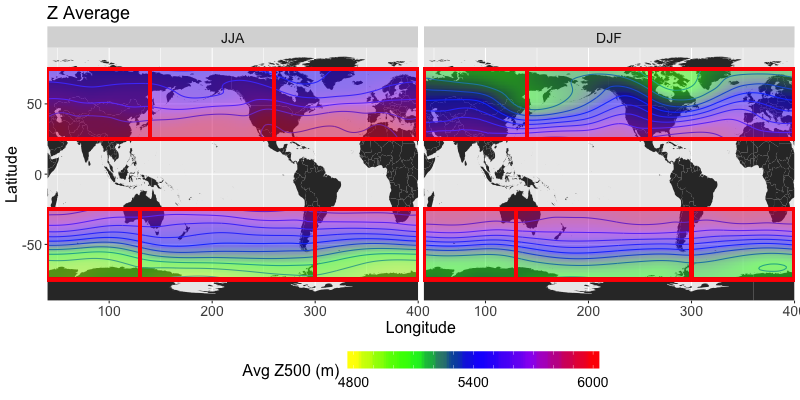
\includegraphics[width=0.75\textwidth]{fig2a}
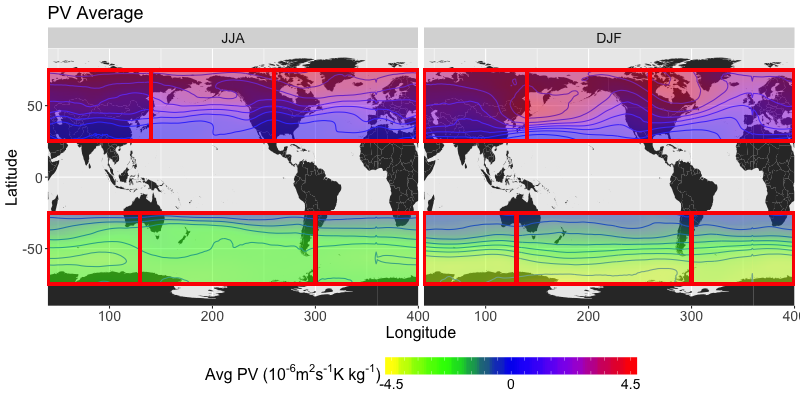
\includegraphics[width=0.75\textwidth]{fig2b}
\caption{Seasonal averages of long term daily mean Z500 (top) and vertically averaged PV (bottom) values for (left) JJA, and (right) DJF, ERA-Interim 1980-2006. Each seasonal average contains 26 years' worth of data. Red rectangles denote the study regions as outlined in Table \ref{geogtable}; from left to right, the NH regions are NC, NP, and NA, and the SH regions are SI, SP, and SA.{\color{teal}R2: What are the blue lines?}{\color{blue}MAR: contour lines-- will specify}}\label{avg}
\end{figure*}



\begin{figure*}
\centering
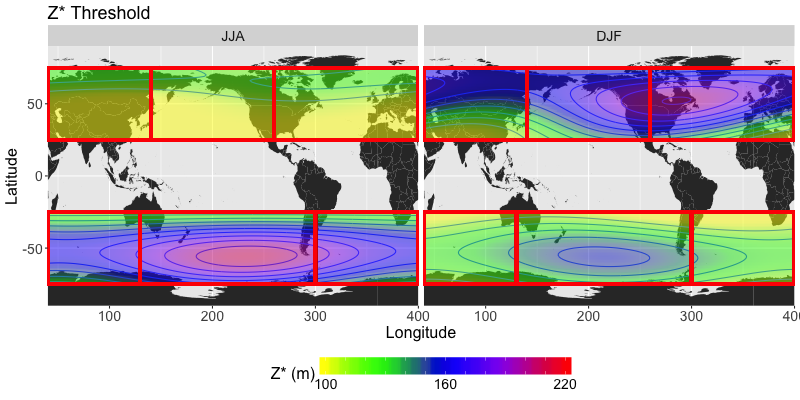
\includegraphics[width=0.75\textwidth]{fig3a}
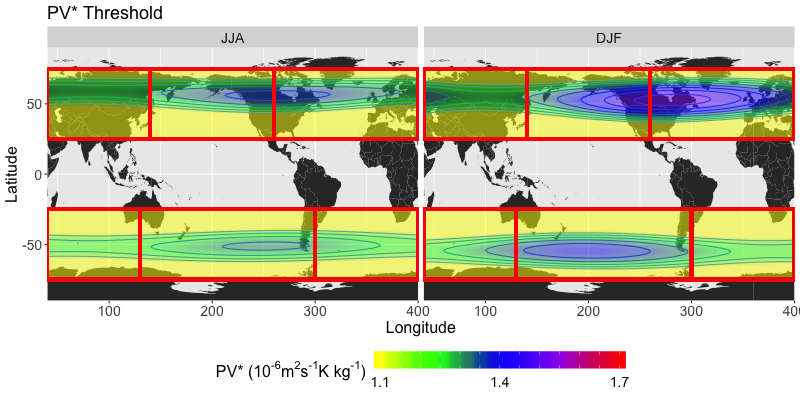
\includegraphics[width=0.75\textwidth]{fig3b}
\caption{Seasonal averages of (top) Z500 anomaly ($Z500^*$) and (bottom) vertically averaged PV anomaly ($VPV^*$) threshold values, as described in Section \ref{modanom}, for (left) JJA and (right) DJF. Red rectangles denote same regions described in Figure \ref{avg} caption.}\label{thresh}
\end{figure*}



\begin{figure*}
\centering
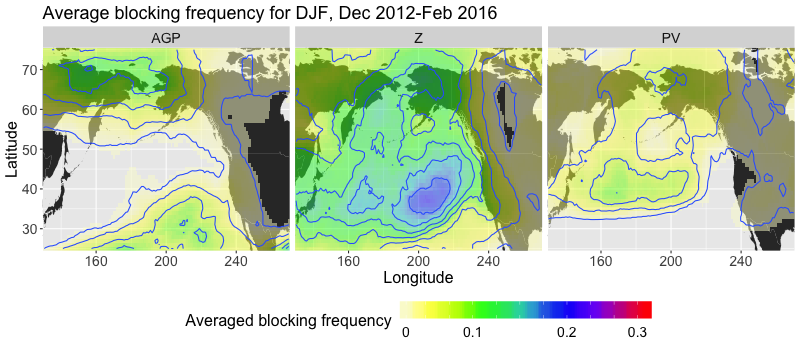
\includegraphics[width=0.75\textwidth]{fig4}
\caption{Long term seasonally averaged blocking frequency for (left) JJA and (right) DJF, (top row) $AGP$ method, (center row), $Z^*$ method, (bottom row) $PV^*$ method. Frequency values represent the fraction of blocked days per season as averaged over the 26 years of the study, with frequencies here ranging from 0.01 (less than one day per season) to 0.27 (about 25 days per season). Contour lines have intervals of 0.03.}\label{blockdens} 
\end{figure*}

\begin{figure*}
\centering
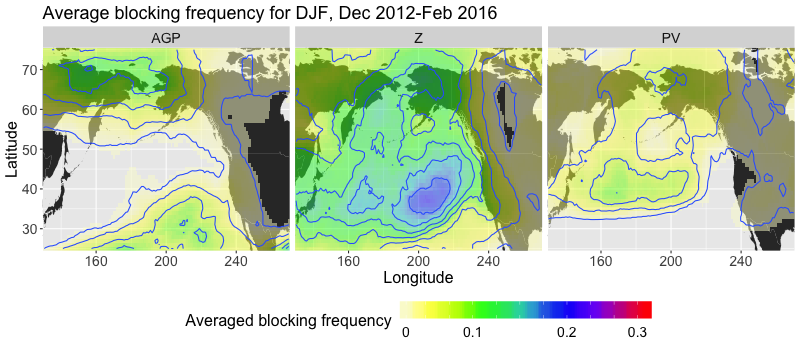
\includegraphics[width=0.85\textwidth]{fig5}
\caption{Blocking frequency, averaged over winters from 2012-2016, for the $AGP$ method (left), $Z^*$ method (center), and $PV^*$ method (right)}\label{RRRFreq}
\end{figure*}

\begin{figure*}
\centering
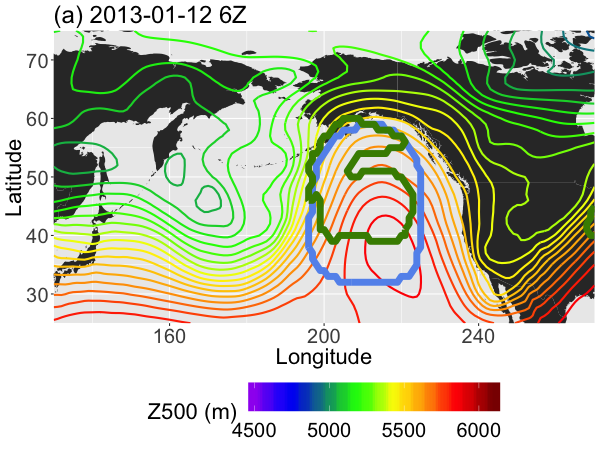
\includegraphics[width=0.38\textwidth]{fig6a}
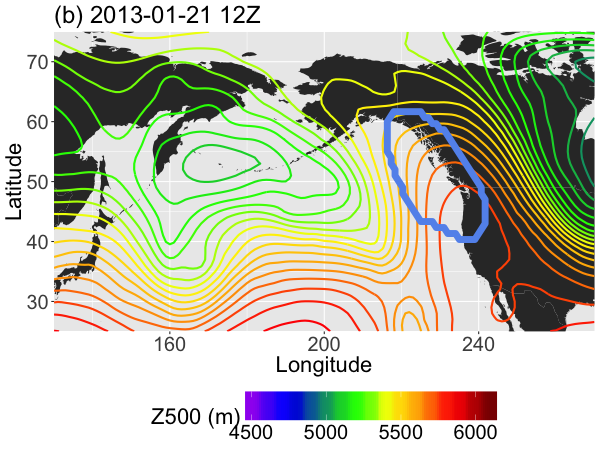
\includegraphics[width=0.38\textwidth]{fig6b}\\
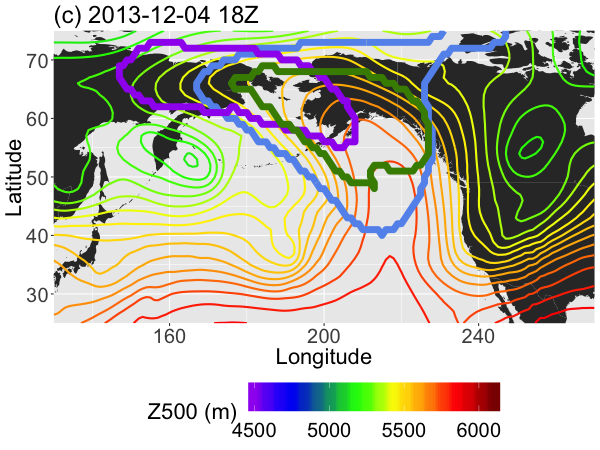
\includegraphics[width=0.38\textwidth]{fig6c}
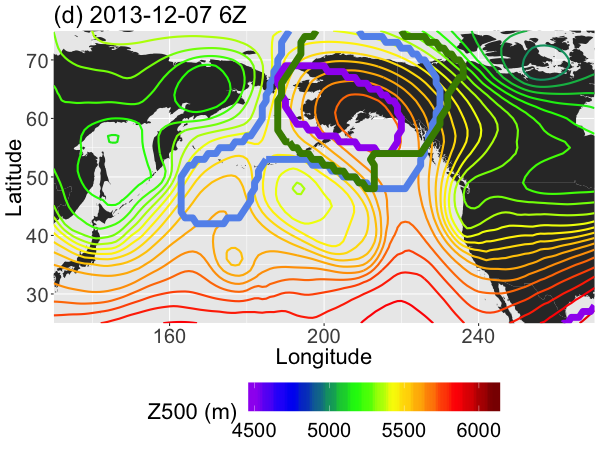
\includegraphics[width=0.38\textwidth]{fig6d}
\caption{(a-b) Examples of ridges that were detected by only the anomaly methods ($Z^*$, blue, and $PV^*$, green) in January 2013. (c-d) Examples of ridges that were detected by all three methods (including $AGP$, purple) in December of 2013.}\label{RRRpanel}
\end{figure*}

\begin{figure*}
\centering
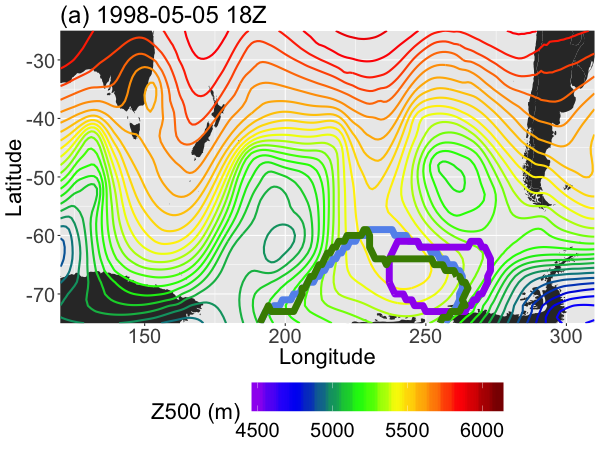
\includegraphics[width=0.38\textwidth]{fig7a}
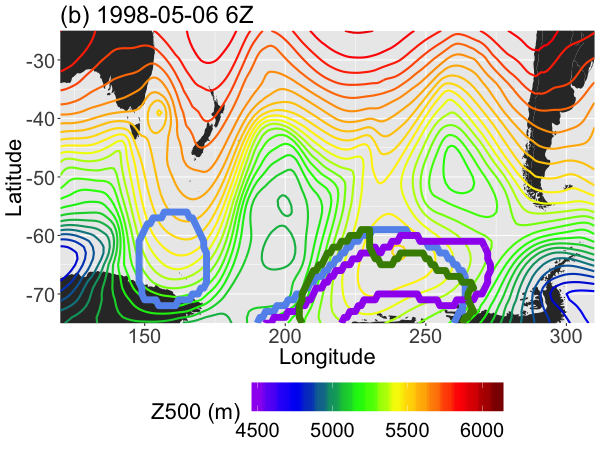
\includegraphics[width=0.38\textwidth]{fig7b}
\caption{Example, 12 hours apart in 1995 MAM, of instances in which there is (a) less and (b) more agreement between the $AGP$ method (purple) and the two anomaly methods (blue and green) in SP.}\label{zgdiff}
\end{figure*}


\begin{figure*}
\centering
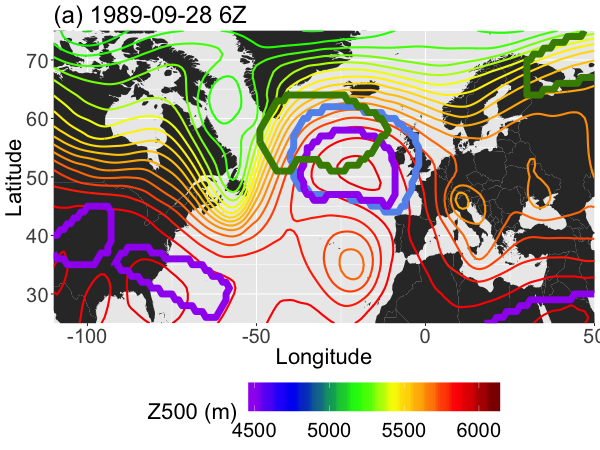
\includegraphics[width=0.38\textwidth]{fig8a}
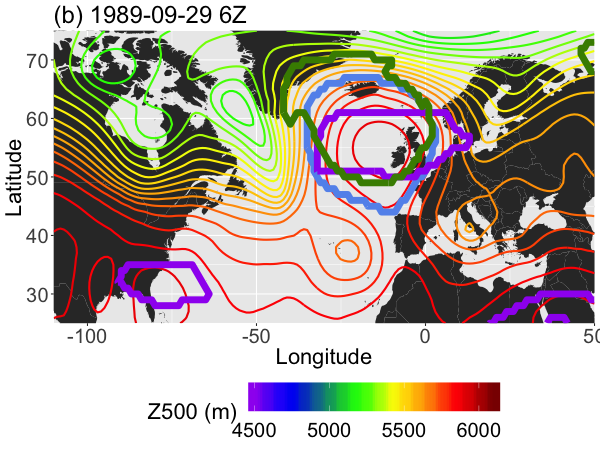
\includegraphics[width=0.38\textwidth]{fig8b}\\
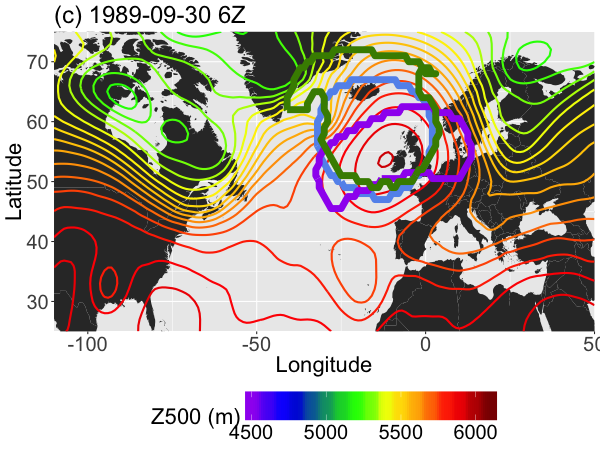
\includegraphics[width=0.38\textwidth]{fig8c}
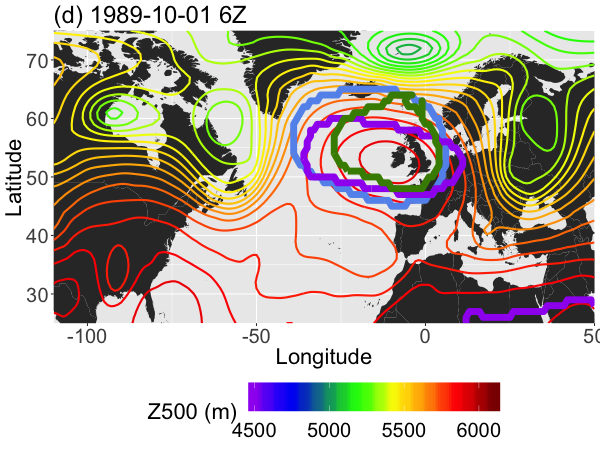
\includegraphics[width=0.38\textwidth]{fig8d}
\caption{Example, in 24-hour increments, of omega block detection in 1989 NA SON. The $PV^*$ method is denoted by the green contour, the $Z^*$ method is blue, and the $AGP$ method is purple.}\label{pvdiff}
\end{figure*}

\begin{figure*}
\centering
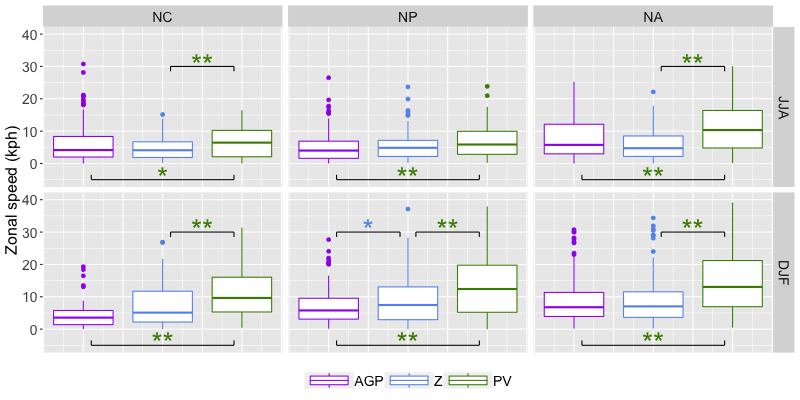
\includegraphics[width=0.38\textwidth]{fig9a}
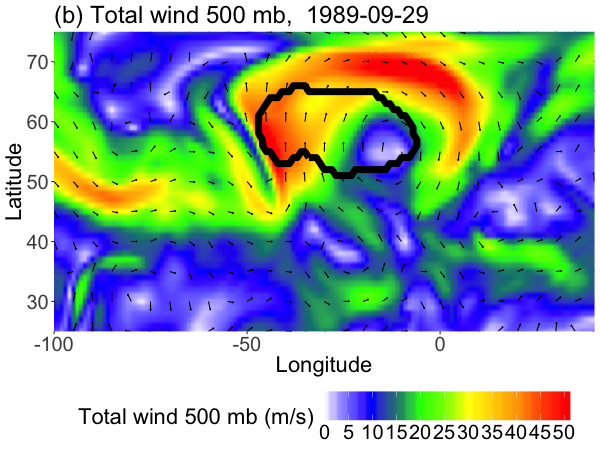
\includegraphics[width=0.38\textwidth]{fig9b}\\
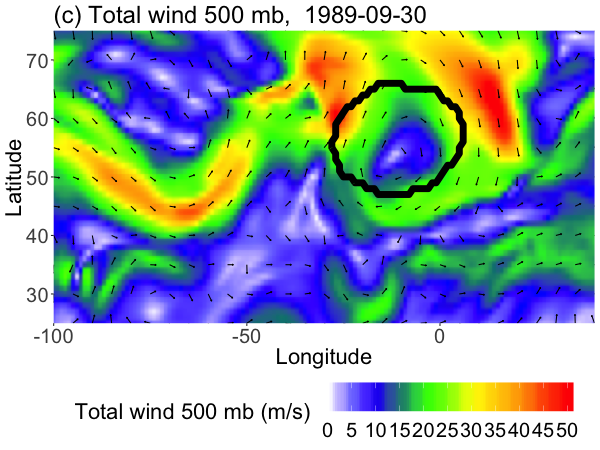
\includegraphics[width=0.38\textwidth]{fig9c}
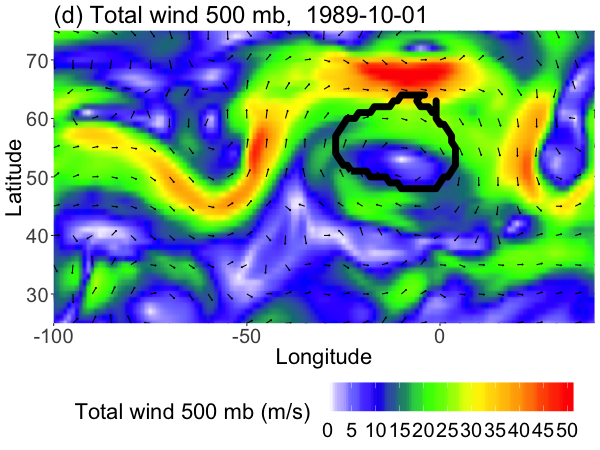
\includegraphics[width=0.38\textwidth]{fig9d}
\caption{500 hPa vector wind field corresponding to previous figure (September 28th-October 1st), showing location of jet streaks. Wind speeds upwards of 45 m/s are visualized as the red areas. The thick black contour corresponds to the blocked region detected by $PV^*$.}\label{windfield}
\end{figure*}





\begin{figure*}
\centering
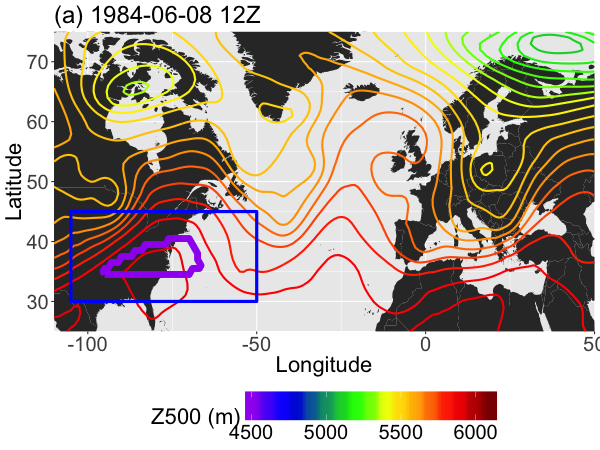
\includegraphics[width=0.38\textwidth]{fig10a}
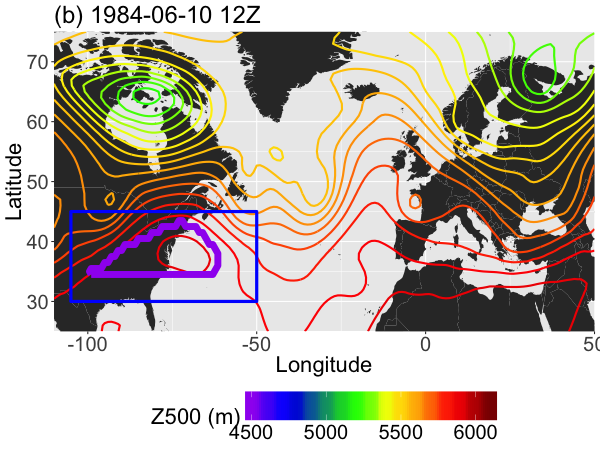
\includegraphics[width=0.38\textwidth]{fig10b}\\
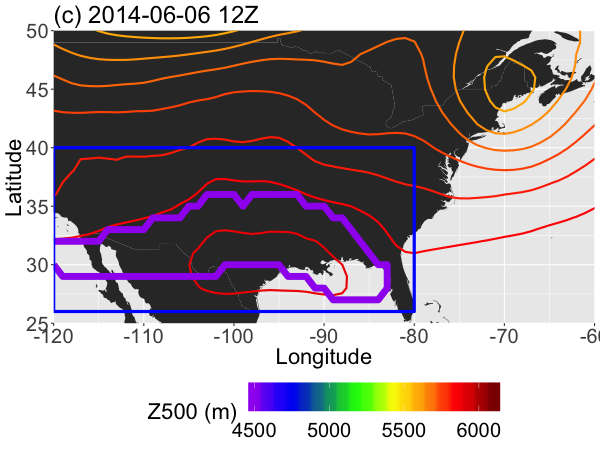
\includegraphics[width=0.38\textwidth]{fig10c}
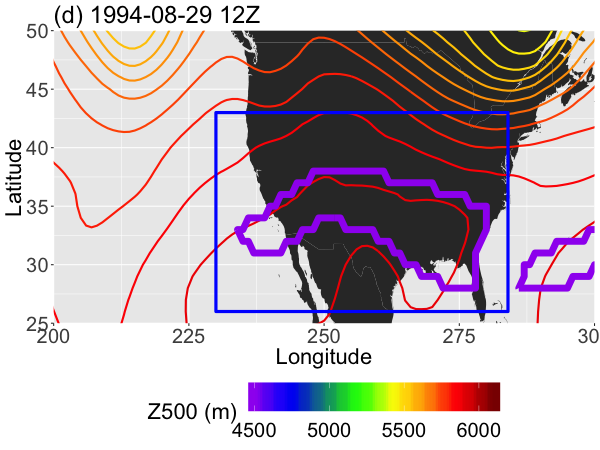
\includegraphics[width=0.38\textwidth]{fig10d}
\caption{Example, in 48-hours increments, from NA JJA 1984, of a low-latitude block detected by the $AGP$ method{ \color{blue}(the other two methods did not detect a block at this time)}. Thin contours are Z500 in 50m intervals, and the thick purple contour denotes the detected feature. The blue box spans [105W-50W, 30N-45N] and outlines the extent of the detected block.{\color{teal}\sout{R2: Are results from the other two methods not included here, or do these two methods not identify any blocking in this case?}}}\label{lowlatjja}
\end{figure*} 



\begin{figure*}
\centering
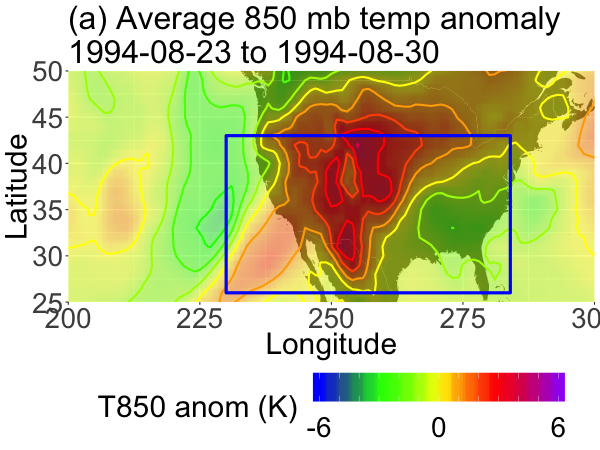
\includegraphics[width=0.25\textwidth]{fig11a}
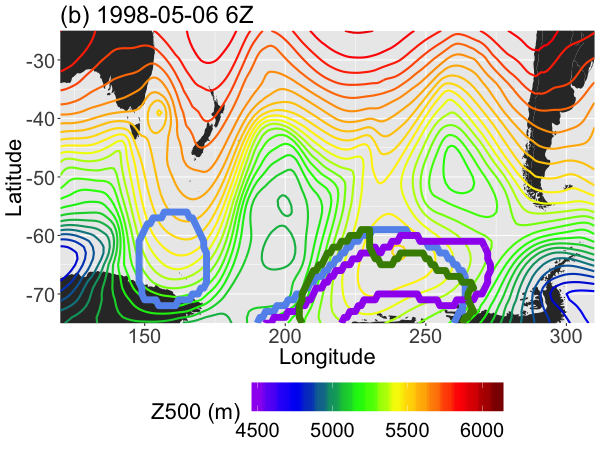
\includegraphics[width=0.25\textwidth]{fig11b}
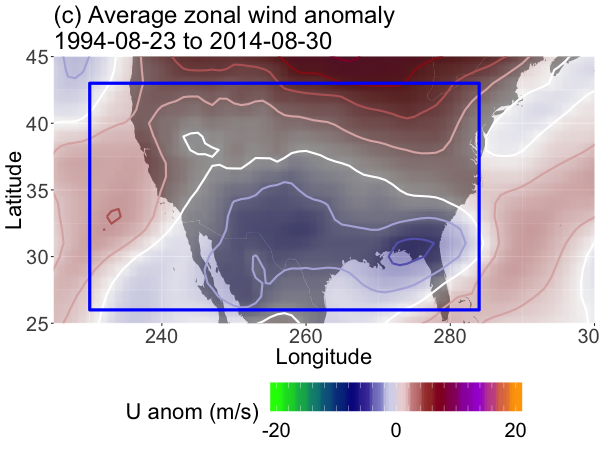
\includegraphics[width=0.25\textwidth]{fig11c}
\caption{Averaged (a) 850 hPa temperature, (b) 500 hPa meridional, and (c) 500 hPa zonal wind anomalies for June 8th-17th 1984. The temperature contour intervals are 1K and the wind contour intervals are 2 m/s. The blue box corresponds to the one seen in Figure \ref{lowlatjja}.}\label{avgjja}
\end{figure*} 

\begin{figure*}
\centering
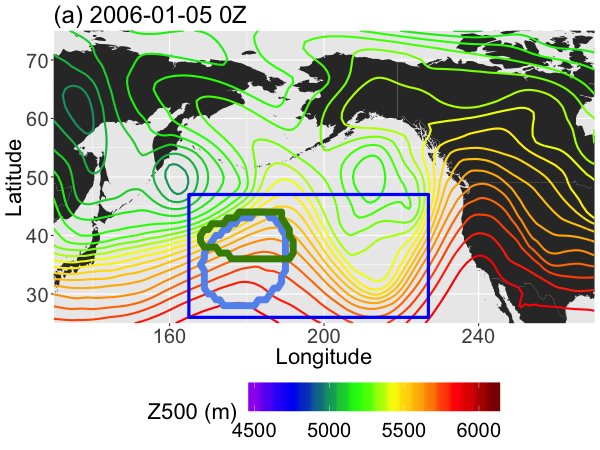
\includegraphics[width=0.37\textwidth]{fig12a}
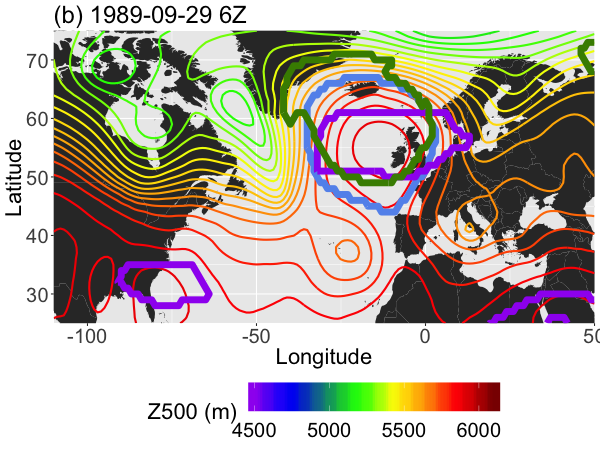
\includegraphics[width=0.37\textwidth]{fig12b}\\
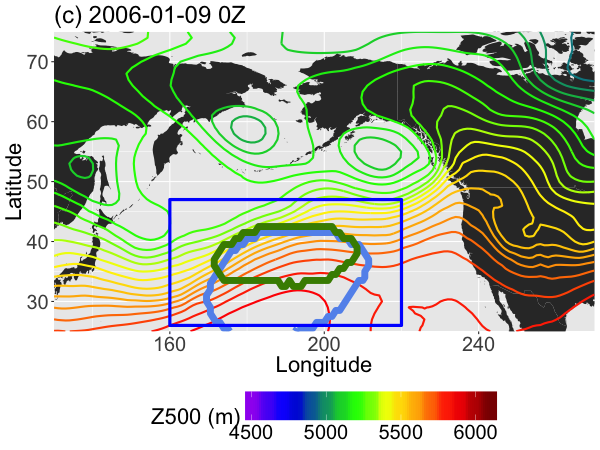
\includegraphics[width=0.37\textwidth]{fig12c}
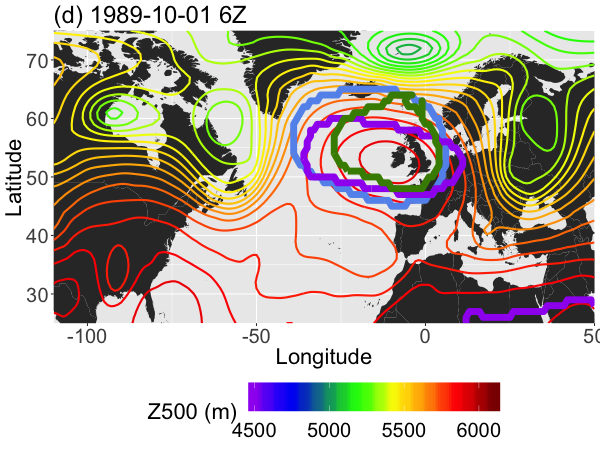
\includegraphics[width=0.37\textwidth]{fig12d}
\caption{Example, in 24-hours increments, from NP DJF 2006, of a low-latitude block detected by the $Z^*$ (blue) and $PV^*$ (green) methods. The blue box spans [160E-220E, 26N-47N] and outlines the extent of the detected block.
}\label{lowlatdjf}
\end{figure*}

\begin{figure*}
\centering
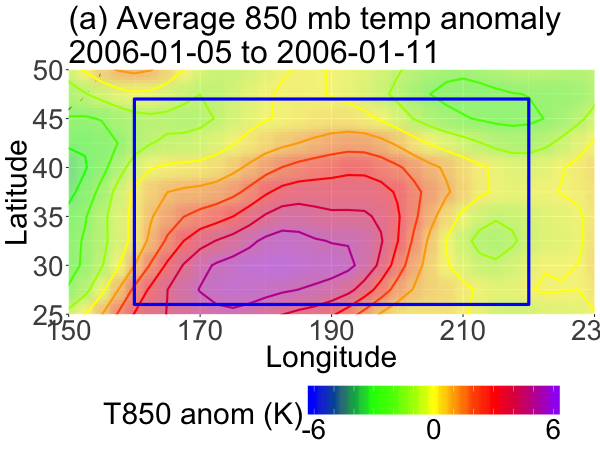
\includegraphics[width=0.25\textwidth]{fig13a}
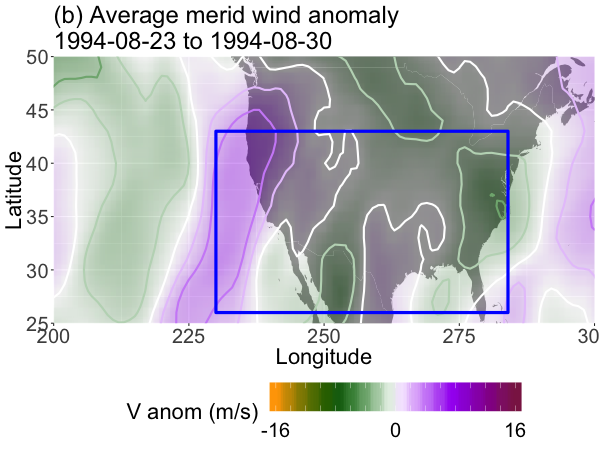
\includegraphics[width=0.25\textwidth]{fig13b}
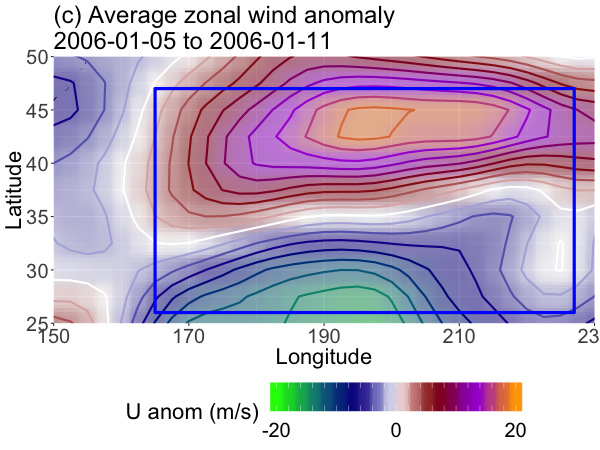
\includegraphics[width=0.25\textwidth]{fig13c}
\caption{Averaged (a) 850 hPa temperature, (b) 500 hPa meridional, and (c) 500 hPa zonal wind anomalies for January 6th-11th 2006. The temperature contour intervals are 1K and the wind contour intervals are 2 m/s. The blue box corresponds to the one seen in Figure \ref{lowlatdjf}}\label{avgdjf}
\end{figure*}

\begin{figure*}
\centering
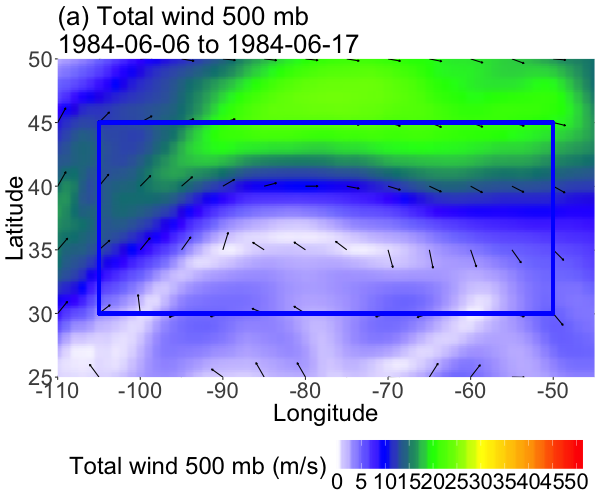
\includegraphics[width=0.37\textwidth]{fig14a}
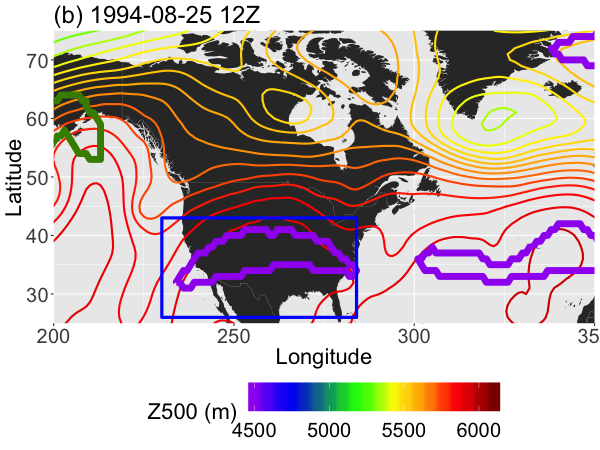
\includegraphics[width=0.37\textwidth]{fig14b}
\caption{500 hPa total wind fields and vectors for (a) the JJA blocking case in Figure \ref{lowlatjja} and (b) the DJF blocking case in Figure \ref{lowlatdjf}. The vectors indicate the wind direction, and the colors indicate the wind magnitude.}\label{totwind}
\end{figure*}


\end{document}
% end of file template.tex